%!TEX program = xelatex
\documentclass[12pt,a4paper]{article}

% Font and encoding
\usepackage{fontspec}
\setmainfont{TeX Gyre Pagella}
\usepackage{microtype}

% Mathematics
\usepackage{amsmath,amssymb,amsthm}
\usepackage{mathtools}

% Layout
\usepackage[margin=1.2in]{geometry}
\usepackage{setspace}
\onehalfspacing

% Section formatting
\usepackage{titlesec}
\titleformat{\section}{\large\bfseries}{\thesection.}{0.8em}{}
\titleformat{\subsection}{\normalsize\bfseries\itshape}{\thesubsection.}{0.6em}{}

% Diagrams
\usepackage{tikz}
\usetikzlibrary{arrows.meta, positioning, calc, decorations.pathreplacing,
                decorations.pathmorphing, shapes.geometric, fit, backgrounds}

\usepackage{pgfplots}
\pgfplotsset{compat=1.18}

% Headers/footers
\usepackage{fancyhdr}
\setlength{\headheight}{14pt}
\pagestyle{fancy}
\fancyhf{}
\fancyhead[L]{\small\itshape A Field-Theoretic Interpretation of the Capital Order}
\fancyhead[R]{\small\thepage}
\renewcommand{\headrulewidth}{0.3pt}

% Hyperref
\usepackage[colorlinks=true, linkcolor=black, citecolor=black, urlcolor=black]{hyperref}

% Theorem environments
\theoremstyle{definition}
\newtheorem{definition}{Definition}[section]
\newtheorem{proposition}{Proposition}[section]
\newtheorem{corollary}{Corollary}[section]
\theoremstyle{remark}
\newtheorem{remark}{Remark}[section]

% Operators
\DeclareMathOperator{\diam}{diam}
\DeclareMathOperator{\tr}{tr}
\DeclareMathOperator*{\argmin}{arg\,min}
\newcommand{\Ct}{\mathcal{C}_t}

% ─────────────────────────────────────────────────
\begin{document}

\begin{titlepage}
  \begin{center}
    \vspace*{2cm}
    {\LARGE\bfseries A Field-Theoretic Interpretation of the Capital Order}\\[1.2em]
    {\large\itshape Formalizing Political Economy after Clara E.\ Mattei}\\[2.5em]
    {\normalsize Flyxion}\\[0.4em]
    {\small standardgalactic.github.io/research-projects}\\[3em]
    {\small March 2026}\\[4em]
    \begin{minipage}{0.78\textwidth}
      \small\itshape
      \textbf{Abstract.} Clara E.\ Mattei's \emph{Escape from Capitalism: An Intervention} argues that the discipline of economics functions as a political technology sustaining a structure of class power she terms the ``capital order.'' This paper provides a formal reconstruction of that argument, extending it with theoretical contributions from Karl Marx, Karl Polanyi, and Nancy Fraser. Drawing on dynamical systems theory and the Relativistic Scalar-Vector Plenum (RSVP) framework, we model the capital order as a feedback-stabilized institutional attractor embedded within a broader socio-ecological phase space. The visible market economy is shown to constitute only the \emph{front-story} of capitalism: its stability depends on a \emph{back-story} of social reproduction, ecological systems, and political authority that the market simultaneously exploits and disavows. The institutional state is extended from a four-component trajectory $\mathcal{C}_t = (L_t, K_t, P_t, I_t)$ to a six-component socio-ecological configuration $\mathcal{E}_t = (L_t, K_t, R_t, N_t, P_t, I_t)$ governed by a transition map with explicit corrective terms. Market dependence is formalized via double-freedom constraints and a labor reproduction equation; capital accumulation is modeled as an autonomous imperative $dM/dt > 0$ imposing a systemic-subject logic on social decision-making; background condition depletion generates a structural crisis tendency expressed through coupled differential inequalities; and boundary struggles are formalized as contested projections between the market submanifold and surrounding institutional domains. The paper concludes by situating the complete framework within RSVP field theory as a controlled non-equilibrium gradient configuration in which transformation requires altering the topology of the institutional constraint manifold.
    \end{minipage}
  \end{center}
\end{titlepage}

\tableofcontents
\newpage

% ─────────────────────────────────────────────────
\section{Introduction: Political Economy as a Formal System}

Clara E.\ Mattei's \emph{Escape from Capitalism: An Intervention} occupies a distinctive position within contemporary political economy. Its central claim is that modern economics is not a neutral descriptive science but an instrument of governance: the discipline constructs conceptual frameworks that legitimize particular policy regimes, present historically contingent social arrangements as natural necessities, and remove fundamental questions about the organization of production and distribution from democratic deliberation. The institutional arrangement that economic expertise sustains is what Mattei calls the \emph{capital order}---a socioeconomic configuration in which private ownership of productive assets and generalized wage dependence reproduce class asymmetries across time.

Mattei's argument inherits from three overlapping intellectual traditions. From Karl Marx she takes the analysis of capitalism as a system of social relations governed by the extraction of surplus value. From Karl Polanyi she draws the insight that markets are not spontaneous natural formations but historically constructed institutional arrangements embedded in political and legal structures. From Thorstein Veblen she adopts the critique of economic ideology: that dominant economic theories function to naturalize contingent institutions by presenting them as expressions of universal laws. What distinguishes her contribution is the historical demonstration that economic expertise has itself functioned as one of the most effective mechanisms of capitalist governance---not merely describing the system from outside but actively participating in its reproduction.

This paper extends Mattei's framework by bringing two further theoretical resources to bear on the formal model. Nancy Fraser's analysis of capitalism as a social totality identifies the \emph{hidden abodes} of social reproduction, ecological systems, and political authority that sustain the visible market economy while remaining systematically excluded from its accounting. This extension requires expanding the institutional state space from a four-component representation capturing the front-story of the market to a six-component socio-ecological configuration that includes the back-story conditions on which the front-story depends. Marx's concept of the \emph{double freedom} of the worker and the \emph{capital circuit} $M \to C \to M'$ are formalized as structural constraints on the institutional trajectory, making the accumulation imperative and its social consequences mathematically precise.

This paper pursues a formal reconstruction of this extended framework. The goal is not to provide a mathematical proof of Mattei's or Fraser's political conclusions but to translate the structural claims of their frameworks into the language of dynamical systems theory and the Relativistic Scalar-Vector Plenum (RSVP) framework. RSVP treats complex systems as fields in which energy, information, and agency flow along gradients maintained by structural asymmetries. When political economy is rendered in this language, capitalism appears not merely as a set of institutions but as a gradient-stabilizing configuration embedded within a broader socio-ecological field: a system that persists because it continuously reproduces asymmetries not only between labor and capital but between the market economy and the background conditions it exploits.

\subsection*{Methodological Note}

The formalism developed here is a modeling tool rather than a replacement for historical or institutional analysis. Equations represent structural claims extracted from Mattei's text; they do not constitute independent empirical predictions. The paper is therefore best understood as a \emph{formal reconstruction}---an exercise in translating a qualitative institutional account into a mathematically structured language in order to expose its internal logic, identify hidden assumptions, and clarify the conditions under which the system could be transformed.

This distinction matters for two reasons. First, it respects the irreducibly historical character of Mattei's argument: no set of differential equations can substitute for the archival evidence she marshals about the collaboration between economists and authoritarian regimes in the interwar period. Second, it clarifies the scope of the formal claims being made here. When we write that austerity is a stabilizing feedback mechanism, we are not predicting quantitative magnitudes; we are asserting that austerity policies have the structural role of a feedback controller within the institutional dynamical system, and that this structural role is what Mattei's historical analysis illuminates.

% ─────────────────────────────────────────────────
\section{Beyond the Trading-Rules Myth: Capitalism as Social Order}
\label{sec:social_order}

\subsection{The Economistic Reduction and its Limits}

A persistent feature of mainstream economic discourse is the reduction of capitalism to a neutral set of exchange rules. In this framing, markets are mechanisms that coordinate the voluntary transactions of self-interested agents; prices are signals carrying information; and the overall system tends toward Pareto-optimal equilibria. The ideological function of this reduction is precisely what Mattei identifies as the central political technology of the capital order: by presenting capitalism as a mechanism rather than a social relation, it removes questions of power, ownership, and distribution from the domain of democratic deliberation.

The inadequacy of this framing becomes visible as soon as one asks how markets are constituted and sustained. Legal regimes must define and enforce property rights; monetary authorities must maintain the medium of exchange; states must guarantee contracts and suppress alternatives to wage labor; cultural institutions must reproduce the dispositions of workers and owners alike. Far from being self-generating, the market is the visible surface of a dense institutional architecture whose structural conditions extend far beyond its own perimeter.

Following Nancy Fraser, we distinguish between the \emph{front-story} of capitalism---the sphere of market exchange and wage labor that occupies most economic analysis---and the \emph{back-story} of background conditions that make the front-story possible. These background conditions include social reproduction, ecological systems, and political authority. The formal development of this paper begins with the front-story as formalized in the Mattei-derived framework. This section situates it within the broader back-story structure.

\subsection{The Extended State Space}

The four-component institutional state $\mathcal{C}_t = (L_t, K_t, P_t, I_t)$ captures the front-story variables with adequate precision for the analysis of austerity, technocracy, and labor discipline. However it treats the conditions enabling the front-story as parameters rather than variables. To formalize Fraser's insight, we extend the state space.

\begin{definition}[Socio-Ecological Configuration]
The full socio-ecological state at time $t$ is a sextuple
\begin{equation}
  \label{eq:full_state}
  \mathcal{E}_t = \bigl(L_t,\, K_t,\, R_t,\, N_t,\, P_t,\, I_t\bigr),
\end{equation}
where $R_t$ denotes the social reproduction complex (care work, education, household labor, subject formation) and $N_t$ denotes the ecological system (energy flows, material resources, absorptive capacity for waste). The transition map on the extended state space is
\begin{equation}
  \mathcal{E}_{t+1} = \tilde{\Phi}(\mathcal{E}_t),
\end{equation}
where $\tilde{\Phi}$ reduces to $\Phi$ on the $(L,K,P,I)$ subspace when $R$ and $N$ are held constant, but in general contains terms reflecting the dynamics of reproduction and ecology.
\end{definition}

The standard economic model considers only the projection $\pi_M : \mathcal{E}_t \to (L_t, K_t)$, treating production as a function $F(K_t, L_t)$ that ignores the dependence of both $K_t$ and $L_t$ on $R_t$ and $N_t$. Capitalism's structural disavowal consists in maintaining this projection institutionally: pricing systems, national accounts, and economic models are constructed so that $R$ and $N$ appear as costless externalities rather than as maintained conditions.

\begin{figure}[ht]
\centering
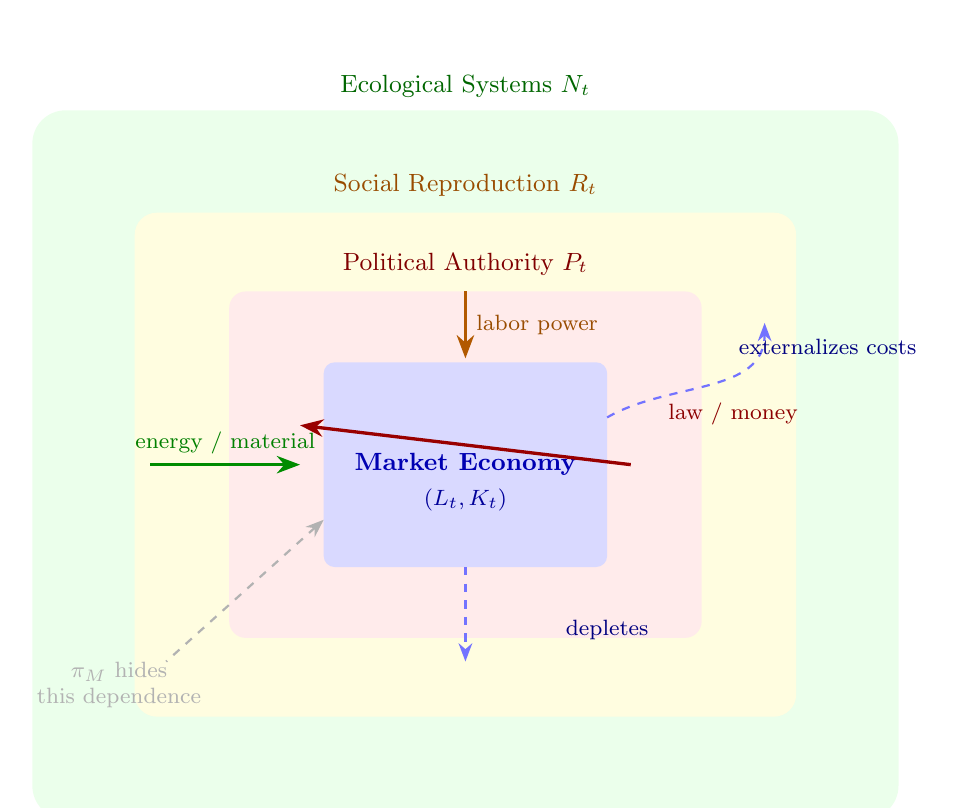
\begin{tikzpicture}[>=Stealth, thick]
  % Outer ecological layer
  \fill[green!8, rounded corners=12pt] (-5.5,-4.5) rectangle (5.5,4.5);
  \node[green!40!black, font=\small] at (0, 4.8) {Ecological Systems $N_t$};

  % Social reproduction layer
  \fill[yellow!12, rounded corners=8pt] (-4.2,-3.2) rectangle (4.2,3.2);
  \node[orange!60!black, font=\small] at (0, 3.55) {Social Reproduction $R_t$};

  % Political layer
  \fill[red!8, rounded corners=6pt] (-3.0,-2.2) rectangle (3.0,2.2);
  \node[red!50!black, font=\small] at (0, 2.55) {Political Authority $P_t$};

  % Market layer (front-story)
  \fill[blue!15, rounded corners=4pt] (-1.8,-1.3) rectangle (1.8,1.3);
  \node[blue!70!black, font=\small\bfseries] at (0, 0) {Market Economy};
  \node[blue!60!black, font=\footnotesize] at (0, -0.45) {$(L_t, K_t)$};

  % Upward arrows: back-story supports front-story
  \draw[->, green!55!black, very thick] (-4.0, 0) -- (-2.1, 0)
    node[midway, above, font=\footnotesize, green!50!black] {energy / material};
  \draw[->, orange!70!black, very thick] (0, 2.2) -- (0, 1.35)
    node[midway, right, font=\footnotesize, orange!60!black] {labor power};
  \draw[->, red!60!black, very thick] (2.1, 0) -- (-2.1, 0.5);
  \node[red!55!black, font=\footnotesize] at (3.4, 0.65) {law / money};

  % Exploitation arrows: market extracts from back-story
  \draw[->, blue!55, dashed] (1.8, 0.6) to[out=30, in=270] (3.8, 1.8);
  \node[blue!50!black, font=\footnotesize] at (4.6, 1.5) {externalizes costs};
  \draw[->, blue!55, dashed] (0, -1.3) to[out=270, in=90] (0, -2.5);
  \node[blue!50!black, font=\footnotesize] at (1.8, -2.1) {depletes};

  % Projection label
  \draw[<-, gray!60, dashed] (-1.8, -0.7) -- (-3.8, -2.5);
  \node[gray!60, font=\footnotesize, align=center] at (-4.4, -2.8) {$\pi_M$ hides\\this dependence};
\end{tikzpicture}
\caption{Layered architecture of the capitalist socio-ecological order. The visible market economy $(L_t, K_t)$ constitutes the front-story. It is sustained by three background layers: social reproduction, political authority, and ecological systems. The market economy extracts from and externalizes costs onto these layers (dashed arrows) while the standard economic projection $\pi_M$ renders the dependence invisible.}
\label{fig:layers}
\end{figure}

% ─────────────────────────────────────────────────
\section{The Double Freedom of the Worker}
\label{sec:double_freedom}

\subsection{A Historically Specific Labor Market}

The capitalist labor market requires a historically specific type of worker whom Marx characterized through the concept of \emph{double freedom}. Workers are doubly free in two senses simultaneously: they possess legal freedom to enter into and dissolve wage contracts, and they are ``freed'' from ownership of the means of subsistence---separated from direct access to land, tools, and common resources that would allow them to survive outside market relations. This double structure is not a universal feature of human labor organization but a historically constructed condition produced through enclosures, colonial dispossession, and the legal reorganization of property.

The formal analysis of survival coupling in Section~\ref{sec:dependence} captures the second dimension of double freedom: the separation from direct means of subsistence that makes market participation compulsory. The first dimension---legal freedom---is equally important to the ideological architecture of the capital order. Because the wage contract is formally voluntary, the coercion built into market dependence is concealed. The worker appears to choose freely to sell labor power; the structural condition making that choice compulsory is rendered invisible.

\subsection{Double Freedom as a Formal Constraint Pair}

The two dimensions of double freedom can be represented as a constraint pair operating on the institutional state.

\begin{definition}[Double Freedom Constraints]
Worker $i$ operates under double freedom when two conditions hold simultaneously:
\begin{align}
  \label{eq:legal_freedom}
  &\text{(Legal freedom):}\quad \exists\, \text{contract}\; c_i \;\text{such that}\; c_i \;\text{is revocable at will by } i, \\
  \label{eq:structural_compulsion}
  &\text{(Structural compulsion):}\quad w_i\bigl(L_i = 0\bigr) < S_i,
\end{align}
where the second condition states that the income available to worker $i$ when supplying zero labor is strictly below the survival threshold. Together these conditions define the double-freedom region of the institutional state space:
\begin{equation}
  \mathcal{D} = \bigl\{\, \mathcal{E} : \eqref{eq:legal_freedom} \;\text{and}\; \eqref{eq:structural_compulsion} \;\text{hold for all }\, i \in L \,\bigr\}.
\end{equation}
\end{definition}

\begin{proposition}[Double Freedom as Ideological Cover]
The intersection $\mathcal{D} \cap \mathcal{S}$ is nonempty and forms a subregion of the capital order's basin of attraction $\mathcal{B}(\mathcal{A}_\mathcal{C})$. Within this region, the legal freedom condition~\eqref{eq:legal_freedom} provides ideological cover for the structural compulsion condition~\eqref{eq:structural_compulsion}: the apparent voluntariness of the wage contract conceals the coercive force of market dependence.
\end{proposition}

The formal significance of this proposition is that the capital order does not require overt coercion to function. The legal framework of free contract is not merely a mask placed over an otherwise brutal system; it is a genuine feature of the institutional configuration that performs a specific stabilizing function. It channels the energies of democratic critique toward the improvement of contract terms rather than toward the transformation of the underlying ownership structure.

\subsection{Institutional Reproduction of the Double-Freedom Condition}

The double-freedom condition is not self-maintaining. It was historically produced through specific processes---enclosures, colonial land expropriation, the destruction of subsistence agriculture---and it must be continuously reproduced through ongoing institutional work. Property law prevents re-enclosure of resources by workers; zoning and planning law restricts subsistence production; intellectual property regimes prevent the non-market distribution of knowledge and technology. Each of these institutional mechanisms contributes a term to the transition map $\tilde{\Phi}$ that reinforces condition~\eqref{eq:structural_compulsion}.

In RSVP terms, the double-freedom condition corresponds to a persistent topological barrier in the social field: a gradient wall preventing the flow of productive resources toward workers that would otherwise reduce their market dependence. Institutional reproduction of this condition means continuously maintaining the barrier against the thermodynamic pressure toward equalization.

% ─────────────────────────────────────────────────
\section{Embedded and Disembedded Markets}
\label{sec:embedding}

\subsection{Polanyi's Double Movement}

Karl Polanyi's analysis in \emph{The Great Transformation} establishes that the self-regulating market is not a natural formation but a political project. Traditional societies embedded market activity within ethical, religious, and political frameworks that constrained the operation of price mechanisms in the interest of social cohesion. Capitalism constructed a qualitatively different arrangement: a disembedded market that claimed autonomy from these frameworks and asserted that the price mechanism should be the primary regulator of social life.

The formal structure of this claim is a claim about the size and character of the set $\Omega_t$ of institutionally admissible configurations. Traditional embedded markets restricted the domain of price-mediated allocation to a subset of the institutional possibility space. The capitalist project expanded this domain, constructing legal, political, and ideological mechanisms to subject ever-larger portions of social life to market allocation.

\begin{definition}[Embedding Degree]
Let $\Omega$ be the full institutional possibility space and $\Omega_{\mathrm{market}}(t) \subseteq \Omega$ the subset of social activities subject to market allocation at time $t$. The embedding degree of the market at $t$ is
\begin{equation}
  \epsilon(t) = \frac{\mathrm{vol}\bigl(\Omega_{\mathrm{market}}(t)\bigr)}{\mathrm{vol}(\Omega)}.
\end{equation}
Traditional societies operate at low $\epsilon$; the capitalist project drives $\epsilon \to 1$ by converting fictitious commodities---labor, land, and money---into objects of market allocation.
\end{definition}

Polanyi's central theoretical claim is that this expansion is inherently self-undermining. As $\epsilon$ increases, the social damage inflicted by market allocation generates political counter-movements demanding protection. He calls this the \emph{double movement}: simultaneous pressure toward market expansion and social resistance to market expansion.

\subsection{The Double Movement as a Coupled Dynamical System}

The double movement can be formalized as a coupled differential system in the embedding degree $\epsilon$ and the counter-movement pressure $Q$.

\begin{definition}[Double Movement Dynamics]
\label{def:double_movement}
Let $\epsilon(t) \in [0,1]$ measure the degree of market disembedding and $Q(t) \geq 0$ measure the amplitude of social counter-movement pressure. The double movement dynamics are:
\begin{align}
  \label{eq:epsilon_dot}
  \dot{\epsilon} &= a\,\epsilon(1-\epsilon) - b\,Q\,\epsilon, \\
  \label{eq:Q_dot}
  \dot{Q} &= c\,\epsilon\,Q - d\,Q,
\end{align}
where $a$ is the rate of capital-driven market expansion, $b$ the damping effect of counter-movement on expansion, $c$ the rate at which market damage generates counter-movement, and $d$ the natural dissipation of counter-movement energy. The system~\eqref{eq:epsilon_dot}--\eqref{eq:Q_dot} is a variant of the Lotka--Volterra predator--prey model, with market expansion playing the role of predator and social resistance playing the role of prey.
\end{definition}

The equilibrium structure of this system determines whether capitalism reaches a stable disembedding level or cycles between expansion and crisis. In the absence of feedback ($b = 0$, $c = 0$), market expansion drives $\epsilon \to 1$ unconstrained. With feedback, a non-trivial equilibrium $(\epsilon^*, Q^*)$ exists when $c\epsilon^* = d$, representing a contested steady state in which market expansion is balanced by ongoing resistance.

\begin{remark}
The Polanyian double movement dynamics~\eqref{eq:epsilon_dot}--\eqref{eq:Q_dot} operate at a different timescale than the short-run austerity feedback cycle~\eqref{eq:bl_ode}. They describe the secular dynamics of institutional embedding rather than the business-cycle dynamics of labor discipline. The two systems are coupled: austerity policies increase $a$ (accelerating disembedding) while democratic counter-movements contribute to $Q$. A complete model of capitalist dynamics would integrate both timescales.
\end{remark}

% ─────────────────────────────────────────────────
\section{Hidden Abodes: Front-Story and Back-Story}
\label{sec:hidden_abodes}

\subsection{The Productive Function of Concealment}

Marx observed that the sphere of market exchange, in which workers freely sell labor power for a fair wage, is the ``Eden of the innate rights of man.'' To understand exploitation, it is necessary to follow the owners of money and labor power below the surface, into the ``hidden abode of production,'' where the real extraction of surplus value occurs. Fraser extends this insight: there are multiple hidden abodes, not just one. Behind the sphere of wage labor lies the hidden abode of social reproduction; behind production lies the hidden abode of ecological throughput; and behind both lies the hidden abode of political authority that enforces property rights and manages monetary systems.

These hidden abodes share a common structural feature: capitalism depends on them while systematically refusing to account for them. Social reproduction is treated as a free good provided naturally by families and communities. Ecological systems are treated as an inexhaustible resource base and an infinite waste sink. State power is treated as an external guarantee whose costs are borne by taxpayers rather than by capital. Each disavowal constitutes a form of structural free-riding that allows the front-story to appear more productive than it actually is.

\subsection{Extended Production Function and Hidden Dependencies}

The standard economic production function $Y = F(K, L)$ can be extended to make the hidden dependencies explicit:
\begin{equation}
  \label{eq:extended_production}
  Y_t = F\bigl(K_t,\, L_t,\, R_t,\, N_t,\, P_t\bigr),
\end{equation}
where $F_{R_t} > 0$, $F_{N_t} > 0$, and $F_{P_t} > 0$: output depends positively on the social reproduction complex, ecological systems, and political authority. The standard model's projection $\pi_M$ that treats $R_t$, $N_t$, and $P_t$ as parameters is therefore not merely a simplification but a structural concealment: it misrepresents the degree to which the visible market economy depends on background conditions whose maintenance it does not fund.

\begin{definition}[Disavowal Ratio]
The disavowal ratio at time $t$ measures the fraction of total production value that depends on unaccounted background conditions:
\begin{equation}
  \delta(t) = 1 - \frac{F(K_t, L_t, 0, 0, 0)}{F(K_t, L_t, R_t, N_t, P_t)}.
\end{equation}
A high disavowal ratio indicates that the front-story is heavily subsidized by back-story conditions. Capitalism's long-run viability requires $\delta(t)$ to remain bounded above zero while the back-story conditions remain available.
\end{definition}

\subsection{Structural Disavowal in RSVP Terms}

In RSVP field theory, the hidden abodes correspond to entropy-density reservoirs that feed the market production field. Social reproduction maintains the human energy density $\varrho_L$ by replenishing labor power between periods of wage employment. Ecological systems maintain the material energy density $\varrho_N$ that production converts into commodities. Political authority maintains the institutional field gradient that keeps property boundaries intact.

The disavowal mechanism corresponds to a one-way coupling in the RSVP flux field: energy flows from the back-story reservoirs into the market production field, but the market field does not direct equivalent flux back into the reservoirs. The result is a structural depletion of $\varrho_R$, $\varrho_N$, and $\varrho_P$ over time---a net entropy drain from the background conditions that, if unchecked, eventually undermines the conditions of possibility for the front-story itself.

% ─────────────────────────────────────────────────
\section{Capital as the Systemic Subject}
\label{sec:capital_subject}

\subsection{The Accumulation Imperative}

A distinctive feature of capitalism identified by Marx and theorized extensively in the tradition of critical political economy is the emergence of capital as what appears to be an autonomous, self-directing subject of economic life. Individual capitalists do not freely choose to accumulate; the competitive dynamics of the market compel accumulation as a condition of survival. A firm that does not reinvest surplus into expanding production will be outcompeted by those that do. The result is an impersonal accumulation dynamic that operates ``behind the backs'' of the participants, subordinating all social purposes to the self-expansion of value.

The formal expression of this imperative is simple but consequential:
\begin{equation}
  \label{eq:accumulation_imperative}
  \frac{dM}{dt} > 0,
\end{equation}
where $M(t)$ denotes the money-value of capital in the circuit of accumulation. The circuit itself takes the classical Marxian form:
\begin{equation}
  \label{eq:capital_circuit}
  M \;\longrightarrow\; C \;\longrightarrow\; M' = M + \Pi,
\end{equation}
where $C$ represents commodity production employing labor and means of production, and $M'$ is the expanded money-value recovered at the end of the circuit.

\begin{definition}[Accumulation Attractor]
The accumulation imperative~\eqref{eq:accumulation_imperative} defines a directional constraint on the trajectories of the institutional dynamical system: the $K_t$ component of $\mathcal{E}_t$ must grow over time. This constraint can be expressed as an invariant of the flow $\tilde\Phi$:
\begin{equation}
  \frac{d}{dt}\,\mathrm{vol}(K_t) > 0 \qquad \text{along trajectories in } \mathcal{B}(\mathcal{A}_\mathcal{C}),
\end{equation}
where $\mathrm{vol}(K_t)$ measures the scale of capital ownership structures.
\end{definition}

\subsection{Compulsory Growth and the Logic of Value}

The compulsory character of accumulation means that capitalism does not merely \emph{permit} growth; it structurally requires it. Firms, financial institutions, and national economies that fail to maintain $dM/dt > 0$ face existential pressure: bankruptcy, credit downgrade, capital flight, or political crisis. This structural compulsion generates what might be called the \emph{law of value}: the principle that social activities are allocated not according to human need but according to their capacity to generate surplus in the accumulation circuit.

In formal terms, the law of value corresponds to a priority ordering over the components of the extended state $\mathcal{E}_t$. The accumulation imperative~\eqref{eq:accumulation_imperative} takes precedence over the maintenance of $R_t$, $N_t$, and $P_t$. Decisions about production, investment, and resource allocation are made primarily according to their impact on $M' - M$ rather than their impact on social reproduction, ecological integrity, or democratic legitimacy.

\begin{proposition}[Value-Priority Ordering]
In the capital order, the components of $\mathcal{E}_t$ are governed by the priority ordering
\begin{equation}
  K_t \;\succ\; L_t \;\succ\; P_t \;\succ\; R_t \;\succ\; N_t,
\end{equation}
in the sense that when institutional decisions force trade-offs between the maintenance of different components, capital accumulation takes precedence over labor welfare, political authority over social reproduction, and all of the above over ecological integrity.
\end{proposition}

\begin{proof}[Sketch]
The ordering follows from the structure of $\tilde\Phi$ under the accumulation constraint~\eqref{eq:accumulation_imperative}. Capital can be maintained at the expense of labor (through wage suppression), labor can be maintained at the expense of political legitimacy (through austerity), and political authority can be maintained at the expense of social reproduction (through welfare cuts). Ecological systems are systematically last in the ordering because their degradation is typically slow enough to remain within the disavowal structure for extended periods.
\end{proof}

\subsection{Capital Circuit as a TikZ Dynamical System}

\begin{figure}[ht]
\centering
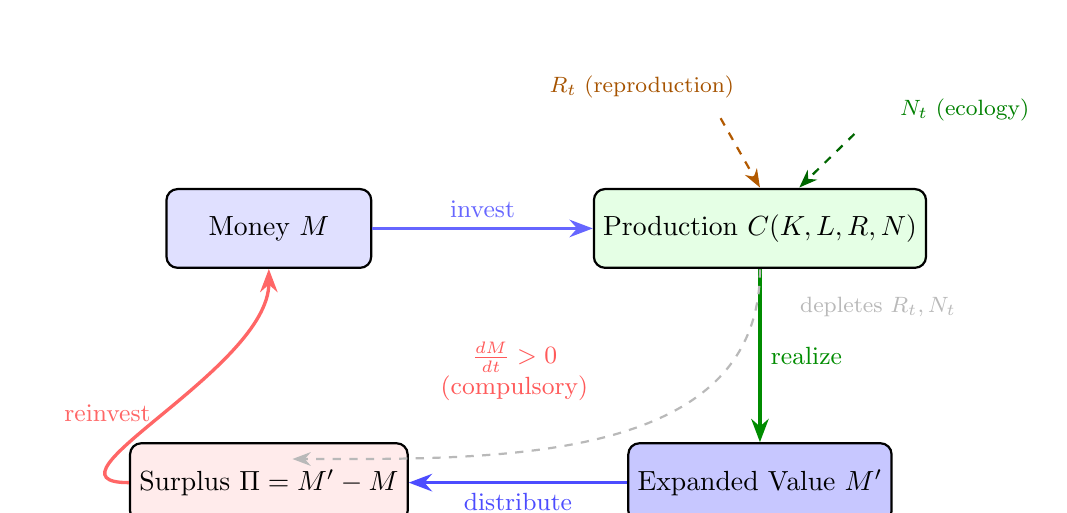
\begin{tikzpicture}[>=Stealth, thick, node distance=2.5cm]
  % Main circuit nodes
  \node[draw, rounded corners, minimum width=2.6cm, minimum height=1.0cm,
        fill=blue!12] (M) {Money $M$};
  \node[draw, rounded corners, minimum width=2.6cm, minimum height=1.0cm,
        fill=green!10, right=2.8cm of M] (C) {Production $C(K,L,R,N)$};
  \node[draw, rounded corners, minimum width=2.6cm, minimum height=1.0cm,
        fill=blue!22, below=2.2cm of C] (Mprime) {Expanded Value $M'$};
  \node[draw, rounded corners, minimum width=2.6cm, minimum height=1.0cm,
        fill=red!8, below=2.2cm of M] (surplus) {Surplus $\Pi = M' - M$};

  % Main circuit arrows
  \draw[->, very thick, blue!60] (M) -- node[above, font=\small] {invest} (C);
  \draw[->, very thick, green!55!black] (C) -- node[right, font=\small] {realize} (Mprime);
  \draw[->, very thick, blue!70] (Mprime) -- node[below, font=\small] {distribute} (surplus);
  \draw[->, very thick, red!60] (surplus) to[out=180, in=270] node[left, font=\small] {reinvest} (M);

  % Imperative annotation
  \node[red!65, font=\small, align=center] at ($(M)!0.5!(Mprime)+(0,-0.2)$)
    {$\frac{dM}{dt} > 0$\\(compulsory)};

  % Background condition flows into production
  \draw[->, orange!70!black, dashed, thick] ($(C)+(-0.5,1.4)$) -- ($(C)+(0,0.52)$);
  \node[orange!65!black, font=\footnotesize] at ($(C)+(-1.5,1.8)$) {$R_t$ (reproduction)};
  \draw[->, green!40!black, dashed, thick] ($(C)+(1.2,1.2)$) -- ($(C)+(0.5,0.52)$);
  \node[green!50!black, font=\footnotesize] at ($(C)+(2.6,1.5)$) {$N_t$ (ecology)};

  % Depletion arrow
  \draw[->, gray!55, dashed] ($(C)+(0,-0.52)$) to[out=270, in=0] ($(surplus)+(0.3,0.3)$);
  \node[gray!55, font=\footnotesize] at ($(C)+(1.5,-1.0)$) {depletes $R_t, N_t$};
\end{tikzpicture}
\caption{The capital accumulation circuit $M \to C \to M'$ as a dynamical attractor. The circuit compels $dM/dt > 0$ regardless of social or ecological consequences. Background conditions $R_t$ (social reproduction) and $N_t$ (ecological systems) feed into production as unaccounted inputs (dashed orange and green arrows), while the circuit simultaneously depletes them. The law of value subordinates all social decisions to the requirements of $\Pi > 0$.}
\label{fig:circuit}
\end{figure}

% ─────────────────────────────────────────────────
\section{Boundary Struggles: The Contested Architecture of Capitalism}
\label{sec:boundary}

\subsection{Fraser's Four Institutional Divisions}

Nancy Fraser identifies four fundamental institutional divisions that structure the capitalist social order. The first is the boundary between the market economy and the sphere of social reproduction: capitalism depends on reproductive labor for the maintenance and renewal of labor power, yet systematically denies its economic character, confining it to the domestic sphere and treating it as a natural gift rather than a produced condition. The second is the boundary between the economy and the polity: capitalism requires political institutions to enforce property rights and manage currency, yet simultaneously demands autonomy from political interference in its operations. The third is the boundary between humanity and nature: the capitalist economy treats ecological systems as an external environment available for unlimited extraction and pollution. The fourth is the division between exploitation and expropriation: alongside the surplus extraction from wage workers, capitalism sustains itself through the expropriation of unpaid or coerced labor from populations excluded from the formal wage relation.

These four divisions are not fixed walls but contested boundaries subject to continuous political struggle. Feminist movements have struggled to make reproductive labor visible and valued. Environmental movements have contested the treatment of nature as a free good. Anti-colonial movements have challenged the expropriation that sustains metropolitan accumulation. Labor movements have continually renegotiated the terms of exploitation. Fraser calls these conflicts \emph{boundary struggles}: disputes not about the distribution of goods within capitalism but about the institutional architecture of capitalism itself.

\subsection{Formal Representation of Boundaries as Projection Constraints}

Each boundary can be formalized as a projection constraint on the extended state space $\mathcal{E}_t$.

\begin{definition}[Boundary Projections]
Define four projection maps from $\mathcal{E}_t$ to submanifolds:
\begin{align}
  \pi_{M/R} &: \mathcal{E}_t \to (L_t, K_t) \quad \text{(hides }R_t\text{: reproduction boundary)}, \\
  \pi_{M/P} &: \mathcal{E}_t \to (L_t, K_t) \quad \text{(hides }P_t\text{: polity boundary)}, \\
  \pi_{M/N} &: \mathcal{E}_t \to (L_t, K_t) \quad \text{(hides }N_t\text{: nature boundary)}, \\
  \pi_{exp} &: \mathcal{E}_t \to \Pi_{\mathrm{wage}} \quad \text{(hides expropriation from non-wage labor)}.
\end{align}
Standard economic analysis operates under the composition $\pi_M = \pi_{M/R} \circ \pi_{M/P} \circ \pi_{M/N}$, suppressing all background conditions simultaneously.
\end{definition}

\begin{definition}[Boundary Struggle as Projection Contest]
A boundary struggle over boundary $b$ is a political contest over whether the projection $\pi_{M/b}$ should be maintained or dissolved. Maintaining the projection preserves the disavowal of background condition $b$; dissolving it forces the costs of maintaining $b$ onto the market accounting of the capital order. Dissolution of projection $\pi_{M/R}$, for instance, would require the capital order to account for the full costs of social reproduction in the pricing of labor power.
\end{definition}

The formal significance of this representation is that boundary struggles are struggles over the geometry of the institutional state space. When a boundary projection is dissolved, the effective dimensionality of the economic model increases and the mapping between market activity and its true social costs becomes more accurate. This increases the cost of maintaining the surplus stability region $\mathcal{S}$: more of the true costs of production become visible, compressing the apparent surplus.

\begin{figure}[ht]
\centering
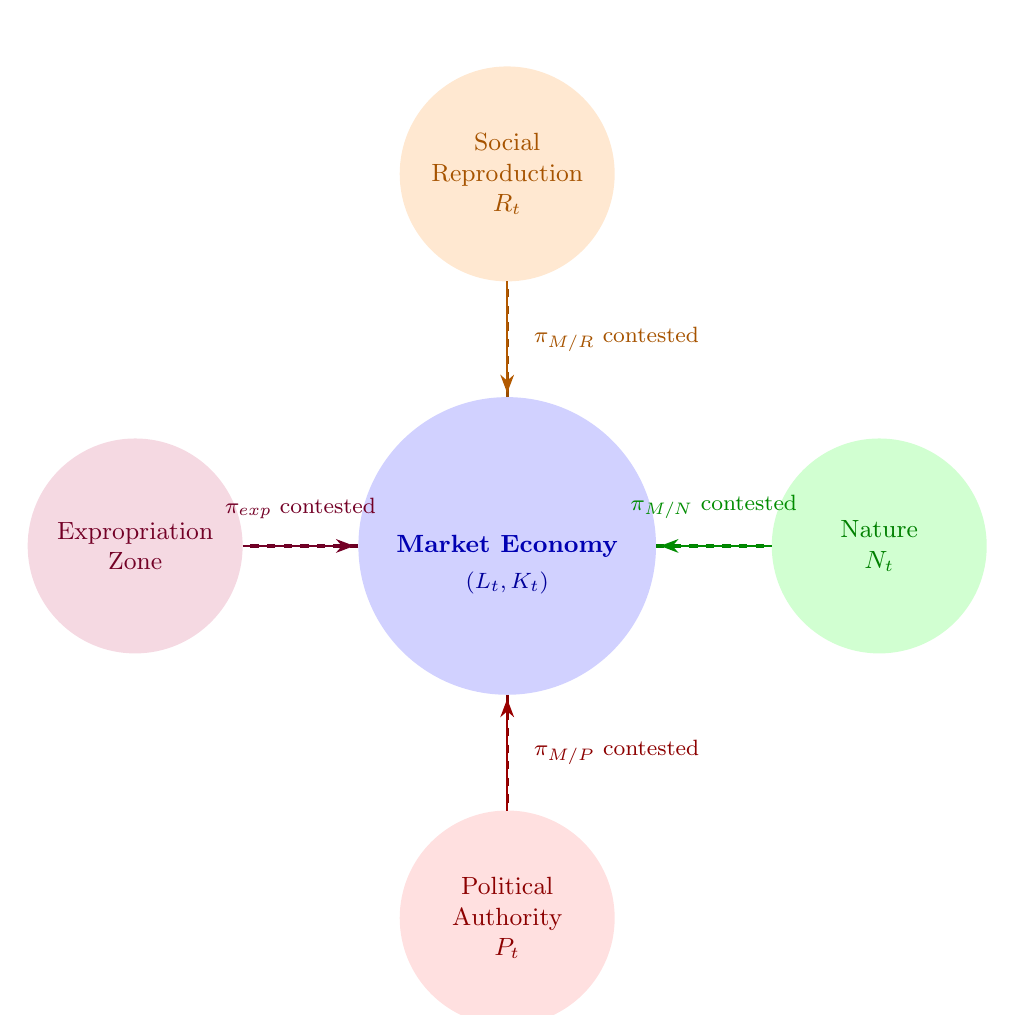
\begin{tikzpicture}[>=Stealth, thick, scale=1.05]
  % Central market circle
  \fill[blue!18] (0,0) circle (1.8cm);
  \node[blue!70!black, font=\small\bfseries] at (0,0) {Market Economy};
  \node[blue!60!black, font=\footnotesize] at (0,-0.45) {$(L_t, K_t)$};

  % Four surrounding domains
  \fill[orange!18] (0, 4.5) circle (1.3cm);
  \node[orange!65!black, font=\small, align=center] at (0, 4.5) {Social\\Reproduction\\$R_t$};

  \fill[green!18] (4.5, 0) circle (1.3cm);
  \node[green!50!black, font=\small, align=center] at (4.5, 0) {Nature\\$N_t$};

  \fill[red!12] (0, -4.5) circle (1.3cm);
  \node[red!55!black, font=\small, align=center] at (0, -4.5) {Political\\Authority\\$P_t$};

  \fill[purple!15] (-4.5, 0) circle (1.3cm);
  \node[purple!60!black, font=\small, align=center] at (-4.5, 0) {Expropriation\\Zone};

  % Boundary lines (contested)
  \draw[very thick, dashed, orange!60!black] (0, 1.8) -- (0, 3.2);
  \draw[very thick, dashed, green!50!black] (1.8, 0) -- (3.2, 0);
  \draw[very thick, dashed, red!50!black] (0, -1.8) -- (0, -3.2);
  \draw[very thick, dashed, purple!55!black] (-1.8, 0) -- (-3.2, 0);

  % Arrows: domains feed market
  \draw[->, orange!70!black, thick] (0, 3.2) -- (0, 1.85);
  \draw[->, green!55!black, thick] (3.2, 0) -- (1.85, 0);
  \draw[->, red!60!black, thick] (0, -3.2) -- (0, -1.85);
  \draw[->, purple!60!black, thick] (-3.2, 0) -- (-1.85, 0);

  % Struggle annotations
  \node[orange!65!black, font=\footnotesize, right] at (0.2, 2.5)
    {$\pi_{M/R}$ contested};
  \node[green!55!black, font=\footnotesize, above] at (2.5, 0.2)
    {$\pi_{M/N}$ contested};
  \node[red!55!black, font=\footnotesize, right] at (0.2, -2.5)
    {$\pi_{M/P}$ contested};
  \node[purple!60!black, font=\footnotesize, above] at (-2.5, 0.2)
    {$\pi_{exp}$ contested};
\end{tikzpicture}
\caption{Fraser's four institutional boundaries as contested projection constraints. The market economy depends on four surrounding domains: social reproduction, nature, political authority, and the expropriation zone. Each dashed boundary represents a projection $\pi$ that hides the dependence. Arrows indicate flows from background domains into the market. Boundary struggles contest whether each projection should be maintained (preserving disavowal) or dissolved (forcing true costs into the accounting of the capital order).}
\label{fig:boundaries}
\end{figure}

% ─────────────────────────────────────────────────
\section{Structural Crisis Tendencies}
\label{sec:crisis}

\subsection{Crises as Background Condition Exhaustion}

Mainstream economic analysis treats crises as aberrations: temporary deviations from a stable equilibrium caused by exogenous shocks, irrational expectations, or policy errors. The framework developed here offers a different interpretation. Because the capital order simultaneously depends on and depletes background conditions---social reproduction, ecological systems, and political legitimacy---it contains endogenous crisis tendencies that do not require exogenous triggers.

This insight follows from combining the accumulation imperative~\eqref{eq:accumulation_imperative} with the extended production function~\eqref{eq:extended_production}. Accumulation drives $Y_t$ upward while simultaneously depleting the background conditions $R_t$, $N_t$, and $P_t$ that sustain production. When depletion outstrips renewal, the background conditions fall below thresholds required for the reproduction of the system.

\begin{definition}[Background Condition Vector]
Let $B_t = (R_t, N_t, P_t)$ denote the vector of background conditions, with each component measured relative to a renewal capacity. Under the accumulation imperative, the dynamics of $B_t$ satisfy:
\begin{align}
  \label{eq:B_dynamics}
  \frac{dB_t}{dt} &= \rho(B_t) - \delta(Y_t, K_t),
\end{align}
where $\rho(B_t) \geq 0$ is the natural renewal rate of background conditions (demographic recovery, ecological regeneration, political legitimacy renewal) and $\delta(Y_t, K_t) > 0$ is the rate of depletion driven by production and accumulation. The capital order requires $dB_t/dt \geq 0$ for at least the interval necessary to reproduce the labor force and maintain productive capacity.
\end{definition}

\begin{proposition}[Structural Crisis Threshold]
There exists a critical threshold $B^* > 0$ such that when $B_t < B^*$, the transition map $\tilde\Phi$ no longer maintains the trajectory within $\mathcal{B}(\mathcal{A}_\mathcal{C})$. Below this threshold, the background conditions are insufficient to reproduce labor power, sustain ecological throughput, or maintain political legitimacy, and the capital order enters structural crisis.
\end{proposition}

\begin{proof}[Sketch]
The production function~\eqref{eq:extended_production} satisfies $F_{R_t}, F_{N_t}, F_{P_t} > 0$, so output falls as background conditions decline. When $B_t$ drops sufficiently, $Y_t$ falls below the level needed to simultaneously satisfy the collective reproduction constraint~\eqref{eq:collective_survival} and the surplus extraction condition~\eqref{eq:surplus}. The bounded reproduction interval~\eqref{eq:bounded_interval} collapses, and the system exits the surplus stability region $\mathcal{S}$.
\end{proof}

\subsection{Three Crisis Modalities}

The crisis threshold proposition implies three distinct modalities corresponding to the three components of $B_t$.

Reproductive crisis occurs when $R_t < R^*$: the social reproduction complex can no longer adequately renew the labor force. This manifests as declining physical and mental health, reduced educational attainment, care deficits, and demographic contraction---all of which reduce the effective supply and productivity of $L_t$.

Ecological crisis occurs when $N_t < N^*$: the ecological system can no longer supply the material inputs or absorb the waste outputs of production at current scale. This manifests as resource depletion, climate disruption, soil degradation, and biodiversity collapse---physical limits that directly constrain the production function.

Legitimation crisis occurs when $P_t < P^*$: political institutions can no longer generate sufficient consent for the capital order among the governed population. This manifests as electoral volatility, institutional delegitimization, and social unrest---conditions under which the technocratic governance mechanisms analyzed in Section~\ref{sec:technocracy} lose their authority.

\begin{figure}[ht]
\centering
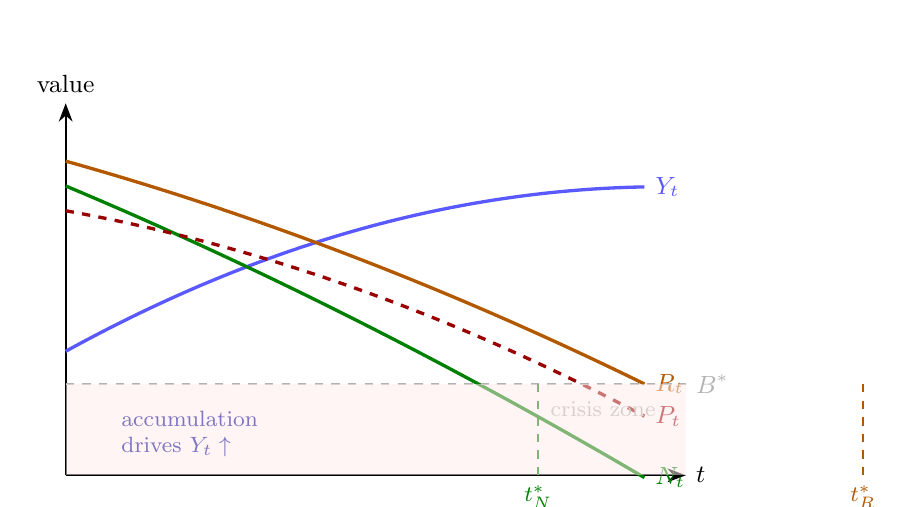
\begin{tikzpicture}[>=Stealth, thick, scale=1.05]
  \draw[->] (0,0) -- (7.5,0) node[right] {\small $t$};
  \draw[->] (0,0) -- (0,4.5) node[above] {\small value};

  % Y growing
  \draw[blue!65, very thick] plot[smooth, domain=0:7, samples=60]
    (\x, {1.5 + 0.55*\x - 0.038*\x*\x})
    node[right] {\small $Y_t$};

  % R_t declining
  \draw[orange!70!black, very thick] plot[smooth, domain=0:7, samples=60]
    (\x, {3.8 - 0.28*\x - 0.015*\x*\x})
    node[right, font=\small] {\small $R_t$};

  % N_t declining faster
  \draw[green!50!black, very thick] plot[smooth, domain=0:7, samples=60]
    (\x, {3.5 - 0.42*\x - 0.012*\x*\x})
    node[right] {\small $N_t$};

  % P_t declining slowly then fast
  \draw[red!60!black, very thick, dashed] plot[smooth, domain=0:7, samples=60]
    (\x, {3.2 - 0.18*\x - 0.025*\x*\x})
    node[right] {\small $P_t$};

  % Critical threshold
  \draw[gray!60, dashed] (0, 1.1) -- (7.5, 1.1)
    node[right, gray!60] {\small $B^*$};

  % Vertical crisis line for N
  \draw[green!50!black, dashed] ({(3.5-1.1)/0.42}, 0) --
    ({(3.5-1.1)/0.42}, 1.1);
  \node[green!50!black, below, font=\footnotesize] at ({(3.5-1.1)/0.42}, 0)
    {$t^*_N$};

  % Vertical crisis line for R
  \draw[orange!70!black, dashed] ({(3.8-1.1)/0.28}, 0) --
    ({(3.8-1.1)/0.28}, 1.1);
  \node[orange!70!black, below, font=\footnotesize] at ({(3.8-1.1)/0.28}, 0)
    {$t^*_R$};

  % Annotation
  \node[blue!60!black, font=\footnotesize, align=left] at (1.5, 0.5) {accumulation\\drives $Y_t\uparrow$};
  \node[gray!60, font=\footnotesize] at (6.5, 0.8) {crisis zone};
  \fill[red!8, opacity=0.5] (0,0) rectangle (7.5, 1.1);
\end{tikzpicture}
\caption{Structural crisis tendency. The accumulation imperative drives $Y_t$ upward while simultaneously depleting background conditions $R_t$ (social reproduction, orange), $N_t$ (ecology, green), and $P_t$ (political legitimacy, dashed red). Each component crosses the critical threshold $B^*$ at a different time ($t^*_N$, $t^*_R$), triggering the corresponding modality of crisis. The crisis zone (shaded) is the region below $B^*$.}
\label{fig:crisis}
\end{figure}

\subsection{Capitalism as a Constrained Socio-Ecological Manifold}

The crisis analysis suggests a further geometric representation of the capital order. Rather than modeling capitalism simply as a trajectory within the four-component institutional state space $\mathcal{X}$, we can represent it as a \emph{constrained submanifold} embedded within the larger socio-ecological phase space $\mathcal{Y}$ spanned by all components of $\mathcal{E}_t$.

\begin{definition}[Capitalist Submanifold]
The capitalist configuration space is the submanifold
\begin{equation}
  \mathcal{M}_{\mathcal{C}} = \bigl\{\, \mathcal{E} \in \mathcal{Y} : w < v_L,\;\; B \geq B^* \,\bigr\}
\end{equation}
defined by the intersection of the surplus stability condition and the background viability condition. The capital order is the dynamical system obtained by restricting $\tilde\Phi$ to $\mathcal{M}_{\mathcal{C}}$. Its structural crisis corresponds to the exit of trajectories from $\mathcal{M}_{\mathcal{C}}$ through the $B < B^*$ boundary rather than through the $w \geq v_L$ boundary.
\end{definition}

\begin{figure}[ht]
\centering
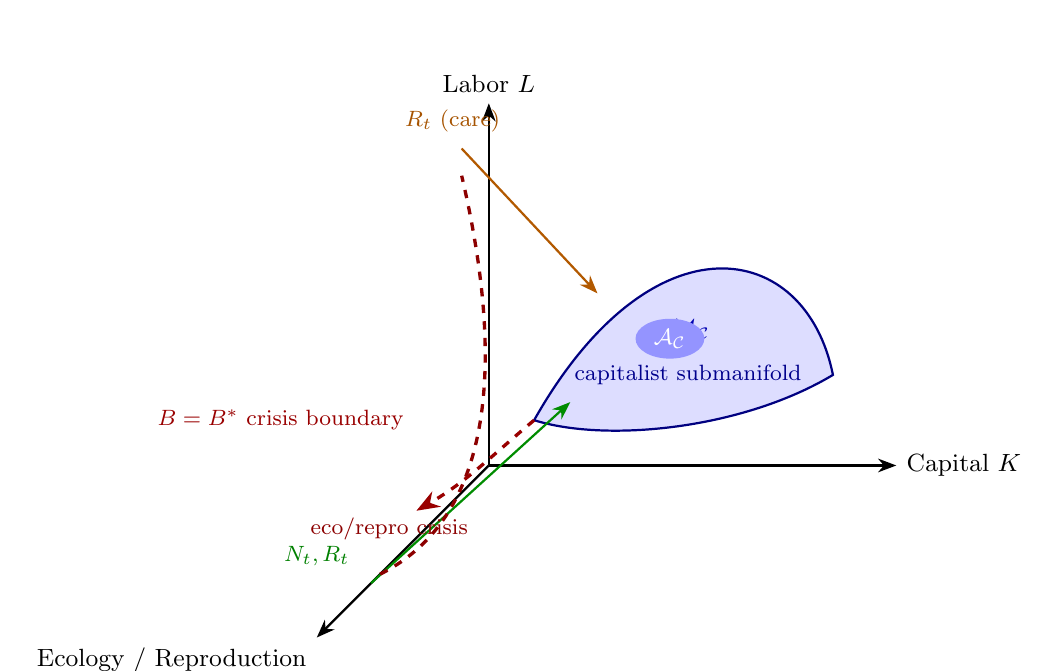
\begin{tikzpicture}[>=Stealth, thick, scale=1.15]
  % Axes
  \draw[->] (0,0,0) -- (4.5,0,0) node[right] {\small Capital $K$};
  \draw[->] (0,0,0) -- (0,4.0,0) node[above] {\small Labor $L$};
  \draw[->] (0,0,0) -- (-1.9,-1.9,0)
    node[below left] {\small Ecology / Reproduction};

  % Capitalist submanifold (shaded region in K-L plane)
  \fill[blue!18, opacity=0.75]
    (0.5, 0.5) .. controls (1.8, 2.8) and (3.5, 2.5) .. (3.8, 1.0)
    .. controls (2.8, 0.4) and (1.3, 0.25) .. (0.5, 0.5);
  \draw[blue!50!black, thick]
    (0.5, 0.5) .. controls (1.8, 2.8) and (3.5, 2.5) .. (3.8, 1.0)
    .. controls (2.8, 0.4) and (1.3, 0.25) .. (0.5, 0.5);
  \node[blue!70!black, font=\small] at (2.2, 1.5) {$\mathcal{M}_\mathcal{C}$};
  \node[blue!55!black, font=\footnotesize] at (2.2, 1.0) {capitalist submanifold};

  % Attractor inside
  \fill[blue!42] (2.0, 1.4) ellipse (0.38cm and 0.22cm);
  \node[white, font=\footnotesize\bfseries] at (2.0, 1.4) {$\mathcal{A}_\mathcal{C}$};

  % Background condition flows (diagonal)
  \draw[->, green!55!black, thick] (-1.3, -1.3) -- (0.9, 0.7);
  \node[green!50!black, font=\footnotesize] at (-1.9, -1.0) {$N_t, R_t$};

  \draw[->, orange!70!black, thick] (-0.3, 3.5) -- (1.2, 1.9);
  \node[orange!65!black, font=\footnotesize] at (-0.4, 3.8) {$R_t$ (care)};

  % Crisis boundary
  \draw[red!55!black, very thick, dashed]
    (-1.2,-1.2) .. controls (0.2, -0.5) and (0.1, 1.5) .. (-0.3, 3.2);
  \node[red!60!black, font=\footnotesize, align=left] at (-2.3, 0.5)
    {$B = B^*$ crisis boundary};

  % Trajectory escaping through crisis boundary
  \draw[->, red!60!black, very thick, dashed]
    (0.5, 0.5) to[out=220, in=30] (-0.8, -0.5);
  \node[red!55!black, font=\footnotesize] at (-1.1, -0.7) {eco/repro crisis};
\end{tikzpicture}
\caption{The capital order as a constrained submanifold $\mathcal{M}_\mathcal{C}$ embedded in the socio-ecological phase space $\mathcal{Y}$. The $K$--$L$ plane represents the visible front-story economy; the diagonal axis represents background conditions (ecology and reproduction). Background condition flows sustain the submanifold (green, orange arrows). The crisis boundary $B = B^*$ (dashed red) defines the lower limit of viability. Trajectories that cross this boundary (red dashed arrow) represent structural crisis driven by background condition exhaustion rather than surplus compression.}
\label{fig:manifold}
\end{figure}

% ─────────────────────────────────────────────────
\section{The Capital Order as a Dynamical Trajectory}
\label{sec:historical}

\subsection{From Static Description to Evolving State Space}

Mattei defines capitalism through the lens of social relations rather than market mechanisms. The defining features of the capital order are: (i) private ownership of productive assets concentrated in a minority class; (ii) generalized wage dependence compelling the majority to sell labor power for subsistence; (iii) systematic extraction of surplus value; and (iv) ideological and institutional reproduction of these conditions across time. The resilience of the capital order does not arise from the intrinsic superiority of capitalist institutions but from the dense network of legal frameworks, policy regimes, professional disciplines, and cultural narratives that continuously reproduce the conditions for capitalist accumulation.

This continuous reproduction is the key insight motivating a dynamical rather than static formalization. The capital order is not a fixed equilibrium; it is a trajectory that must be actively maintained.

\begin{definition}[Institutional State and Trajectory]
The institutional state at time $t$ is a quadruple
\begin{equation}
  \mathcal{C}_t = (L_t,\, K_t,\, P_t,\, I_t),
\end{equation}
where $L_t$ is the labor population endowed with productive capacity; $K_t$ is the capital ownership structure; $P_t$ is the set of active policy institutions and their current parameters; and $I_t$ is the prevailing informational and ideological configuration, including economic theory and professional norms. Each component is a submanifold of the institutional state space $\mathcal{X}$, and the four submanifolds interact through coupling relations specified below.

The institutional trajectory is governed by a transition map
\begin{equation}
  \label{eq:transition}
  \mathcal{C}_{t+1} = \Phi(\mathcal{C}_t),
\end{equation}
where $\Phi : \mathcal{X} \to \mathcal{X}$ encodes the combined effect of economic reproduction, policy feedback, and ideological stabilization. Crucially, $\Phi$ contains correction terms designed to return the trajectory toward the surplus stability region whenever it deviates.
\end{definition}

\subsection{The Surplus Stability Region and its Attractor}

The transition map $\Phi$ is designed---through the historical accumulation of legal, institutional, and ideological mechanisms---to keep trajectories within a specific region of $\mathcal{X}$.

\begin{definition}[Surplus Stability Region]
\label{def:stability_region}
Let $w_t$ denote the aggregate wage rate and $v_L$ the per-unit value produced by labor. The surplus stability region is
\begin{equation}
  \label{eq:surplus}
  \mathcal{S} = \bigl\{\, \mathcal{C} \in \mathcal{X} : w < v_L \,\bigr\},
\end{equation}
the open half-space in which surplus extraction $\Pi = v_L - w > 0$ is maintained. Mattei's claim that the capital order must be actively maintained corresponds to the assertion that $\Phi$ contains feedback terms that push $\mathcal{C}_t$ back into $\mathcal{S}$ whenever $w_t \to v_L$.
\end{definition}

\begin{definition}[Capital Attractor]
The capital attractor is a compact invariant set $\mathcal{A}_\mathcal{C} \subset \mathcal{S}$ such that for any initial condition $\mathcal{C}_0$ in a neighborhood $U(\mathcal{A}_\mathcal{C})$,
\begin{equation}
  d\!\bigl(\Phi^n(\mathcal{C}_0),\, \mathcal{A}_\mathcal{C}\bigr) \to 0 \quad \text{as } n \to \infty,
\end{equation}
where $d$ is the metric on $\mathcal{X}$. The basin of attraction
\begin{equation}
  \mathcal{B}(\mathcal{A}_\mathcal{C}) = \bigl\{\,\mathcal{C}_0 \in \mathcal{X} : \Phi^n(\mathcal{C}_0) \to \mathcal{A}_\mathcal{C}\bigr\}
\end{equation}
is the region of institutional state space from which trajectories converge to capitalist reproduction under $\Phi$.
\end{definition}

The capital order is therefore not characterized by a single static configuration but by an attractor within the surplus stability region toward which the dynamics of the system continually return. Shocks, crises, and democratic challenges perturb trajectories within $\mathcal{B}(\mathcal{A}_\mathcal{C})$ but do not destroy the capital order unless the trajectory exits the basin entirely. This formalizes the resilience that Mattei repeatedly documents historically.

\begin{figure}[ht]
\centering
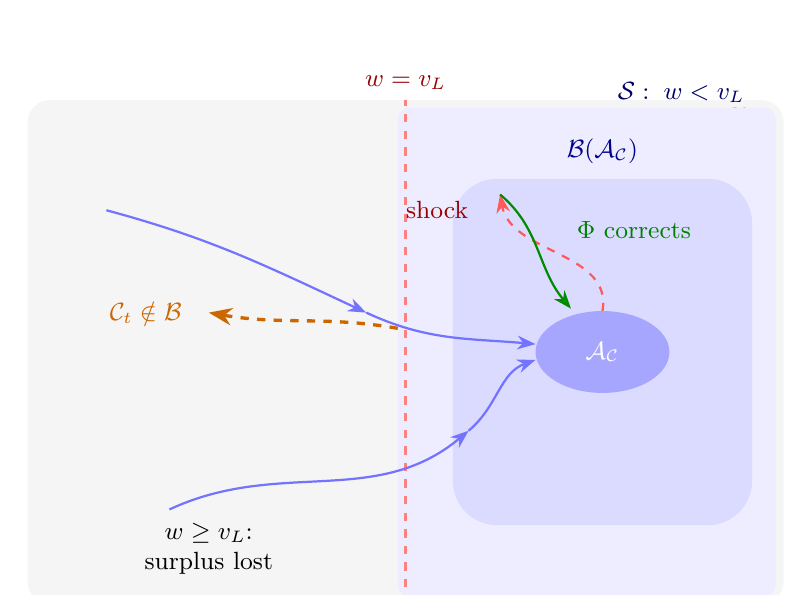
\begin{tikzpicture}[>=Stealth, thick]
  % State space background
  \fill[gray!8, rounded corners=8pt] (-4.8,-3.2) rectangle (4.8,3.2);
  \node[gray!50] at (4.2,3.0) {\small $\mathcal{X}$};

  % Surplus stability region S (right half)
  \fill[blue!7, rounded corners=4pt] (-0.1,-3.1) rectangle (4.7,3.1);
  \node[blue!40!black] at (3.5, 3.3) {\small $\mathcal{S}:\; w < v_L$};

  % Basin of attraction inside S
  \fill[blue!14, rounded corners=16pt] (0.6,-2.2) rectangle (4.4,2.2);
  \node[blue!55!black] at (2.5, 2.55) {\small $\mathcal{B}(\mathcal{A}_\mathcal{C})$};

  % Attractor
  \fill[blue!35] (2.5,0) ellipse (0.85cm and 0.52cm);
  \node[white, font=\small\bfseries] at (2.5,0) {$\mathcal{A}_\mathcal{C}$};

  % Boundary w = v_L
  \draw[red!50, very thick, dashed] (0,-3.2) -- (0,3.2)
    node[above, red!60!black] {\small $w = v_L$};

  % Trajectories converging into basin
  \draw[->, blue!55] (-3.8, 1.8) to[out=-15, in=155] (-0.5, 0.5);
  \draw[->, blue!55] (-0.5, 0.5) to[out=-25, in=175] (1.65, 0.1);

  \draw[->, blue!55] (-3.0, -2.0) to[out=25, in=220] (0.8, -1.0);
  \draw[->, blue!55] (0.8, -1.0) to[out=40, in=200] (1.65, -0.1);

  % Perturbation and corrective return
  \draw[->, red!65, dashed] (2.5, 0.52) to[out=80, in=280] (1.2, 2.0);
  \draw[->, green!55!black] (1.2, 2.0) to[out=320, in=130] (2.1, 0.55);
  \node[red!60!black, font=\small] at (0.4, 1.8) {shock};
  \node[green!50!black, font=\small] at (2.9, 1.55) {$\Phi$ corrects};

  % Trajectory that escapes
  \draw[->, orange!80!black, dashed, very thick] (-0.1, 0.3) to[out=170, in=-10] (-2.5, 0.5);
  \node[orange!80!black, font=\small] at (-3.3, 0.5) {$\mathcal{C}_t \notin \mathcal{B}$};

  % Annotation
  \node[font=\small, align=center] at (-2.5, -2.5) {$w \ge v_L$:\\surplus lost};
\end{tikzpicture}
\caption{The capital order as a metastable attractor $\mathcal{A}_\mathcal{C}$ confined within the surplus stability region $\mathcal{S}$. The transition map $\Phi$ contains correction terms that return perturbed trajectories (red) toward $\mathcal{A}_\mathcal{C}$ (green). Only trajectories that cross the boundary $w = v_L$ or otherwise exit the basin $\mathcal{B}(\mathcal{A}_\mathcal{C})$ represent genuine systemic transformation (orange).}
\label{fig:attractor}
\end{figure}

% ─────────────────────────────────────────────────
\section{Market Dependence: Individual Coupling and Collective Reproduction}
\label{sec:dependence}

\subsection{Individual Survival Coupling}

Mattei's concept of market dependence refers to the structural condition in which most individuals lack direct access to productive resources and must participate in labor markets to secure subsistence. This is enforced through property law, the organization of production, and the enclosure of common resources---not merely an empirical description but a structural constraint built into $\mathcal{C}_t$.

Let the survival requirement of individual $i$ at time $t$ be $S_i > 0$. Income through wage employment is $w_i(t)$. The survival-coupling constraint is:
\begin{equation}
  \label{eq:individual_survival}
  w_i(t) \geq S_i \qquad \forall\, i \in L_t.
\end{equation}
In the capital order, access to resources outside the wage relation is institutionally foreclosed, so constraint~\eqref{eq:individual_survival} is binding: participation in labor markets is the only viable route to subsistence. This coupling is the mechanism through which the biological energy requirements of workers are converted into systematic participation in the production field.

\subsection{Collective Reproduction Constraint}

At the aggregate level, the labor population must reproduce itself biologically and socially for the system to continue operating. This yields a global constraint:
\begin{equation}
  \label{eq:collective_survival}
  W(t) \;:=\; \sum_i w_i(t) \;\geq\; S(t) \;:=\; \sum_i S_i,
\end{equation}
which ensures that aggregate wages are sufficient for the labor population to reproduce. The critical feature of the capital order is that condition~\eqref{eq:collective_survival} can be satisfied simultaneously with the surplus extraction condition $W(t) < Y(t)$, where $Y(t)$ is total output. The system therefore operates inside a \emph{bounded reproduction interval}:
\begin{equation}
  \label{eq:bounded_interval}
  S(t) \;\leq\; W(t) \;<\; Y(t).
\end{equation}

\begin{proposition}[Bounded Exploitation Zone]
There exists a nonempty open region $\mathcal{R} \subset \mathbb{R}^2_+$ in the $(W, Y)$ plane such that both constraints~\eqref{eq:collective_survival} and the surplus inequality $W < Y$ are simultaneously satisfied. The capital order requires institutional parameters to keep $\bigl(W(t), Y(t)\bigr) \in \mathcal{R}$ for all $t$.
\end{proposition}

\begin{proof}[Sketch]
Set $\mathcal{R} = \{(W,Y) : S \leq W < Y\}$. This set is nonempty whenever $Y > S$, which holds under any productive technology whose output exceeds bare subsistence. The lower bound ensures labor reproduction; the upper bound ensures positive surplus. Both are simultaneously satisfiable, and the institutional task of the capital order is precisely to manage $W(t)$ so that it remains in the interior of this interval.
\end{proof}

\subsection{Labor Reproduction Equation}

The survival-coupling constraint implies that the size and composition of the labor population at time $t+1$ depends on the adequacy of wages at time $t$. We model this explicitly:
\begin{equation}
  \label{eq:labor_repro}
  L_{t+1} = R\!\bigl(L_t,\, W(t),\, S(t)\bigr),
\end{equation}
where $R$ is a reproduction function satisfying $\partial R / \partial W > 0$ (higher wages support more robust labor reproduction) and $\partial R / \partial S < 0$ (rising survival costs erode reproduction unless wages keep pace). The capital order requires $W(t)$ to be managed so that $L_{t+1} \approx L_t$: the labor supply must remain sufficiently large to continue serving as an input to production. Equation~\eqref{eq:labor_repro} clarifies that the collective constraint~\eqref{eq:collective_survival} is not merely a static inequality but a dynamical requirement: insufficient wages at $t$ deplete the labor population at $t+1$, undermining the system's own reproduction.

\begin{remark}
Equation~\eqref{eq:labor_repro} also captures the upper bound of the capital order's management problem. If wages grow too close to $v_L$, surplus extraction fails. If wages fall too far below $S$, labor reproduction is undermined. The system must navigate this corridor---maintaining labor viability while preserving the surplus gradient---through the feedback mechanisms analyzed in subsequent sections.
\end{remark}

% ─────────────────────────────────────────────────
\section{Class Structure and the Distribution of Output}
\label{sec:class}

\subsection{Production as a Politically Mediated Process}

Let total economic output be generated by a production function:
\begin{equation}
  Y_t = F(K_t, L_t), \qquad F_K, F_L > 0.
\end{equation}
In neoclassical economics, the distribution of $Y_t$ between labor and capital is treated as a technological fact: wages equal the marginal product of labor, and profit equals the marginal product of capital. Mattei's argument, following the classical political economy tradition, is that this distribution is not determined by technology alone but by the institutional rules governing property rights, bargaining power, and market structure. The production function $F$ determines total output; the distributional outcome depends on $\mathcal{C}_t$.

We write:
\begin{align}
  Y_t &= W(t) + \Pi(t), \\
  W(t) &= \alpha(\mathcal{C}_t) \cdot Y_t, \\
  \Pi(t) &= \bigl(1 - \alpha(\mathcal{C}_t)\bigr) \cdot Y_t,
\end{align}
where $\alpha(\mathcal{C}_t) \in (0,1)$ is the labor share of output, itself a function of the full institutional configuration. The surplus $\Pi(t)$ is therefore a \emph{derived variable} determined by institutional constraints embedded in $\mathcal{C}_t$, not by technological necessity. Mattei's claim that the distribution of output is politically mediated is encoded precisely in the dependence of $\alpha$ on the institutional state.

\subsection{Bargaining Power and the Unemployment Gradient}

The labor share $\alpha(\mathcal{C}_t)$ is primarily governed by labor bargaining power $B_L(t)$. Define:
\begin{equation}
  B_L(t) = B_L\!\bigl(u(t),\, \theta(t)\bigr),
\end{equation}
where $u(t)$ is the unemployment rate and $\theta(t)$ captures institutional parameters (union rights, employment protection, welfare provision). The key structural relations are:
\begin{align}
  \frac{\partial B_L}{\partial u} &< 0 \label{eq:bl_u} \qquad\text{(unemployment weakens labor)},\\
  \frac{\partial \alpha}{\partial B_L} &> 0 \label{eq:alpha_bl} \qquad\text{(bargaining power raises wage share)},\\
  \frac{\partial \Pi}{\partial B_L} &< 0 \label{eq:pi_bl} \qquad\text{(bargaining power compresses surplus)}.
\end{align}
Combining \eqref{eq:bl_u} and \eqref{eq:pi_bl} yields the structural chain:
\begin{equation}
  \label{eq:gradient_chain}
  \frac{\partial \Pi}{\partial u} = \frac{\partial \Pi}{\partial B_L} \cdot \frac{\partial B_L}{\partial u} > 0,
\end{equation}
expressing the formal claim that higher unemployment raises profit rates through reduced bargaining power. This chain is the mathematical content of Mattei's argument that unemployment functions as a disciplinary mechanism within the capital order---not a passive outcome of market forces but an active component of the system's gradient-maintaining machinery.

\begin{figure}[ht]
\centering
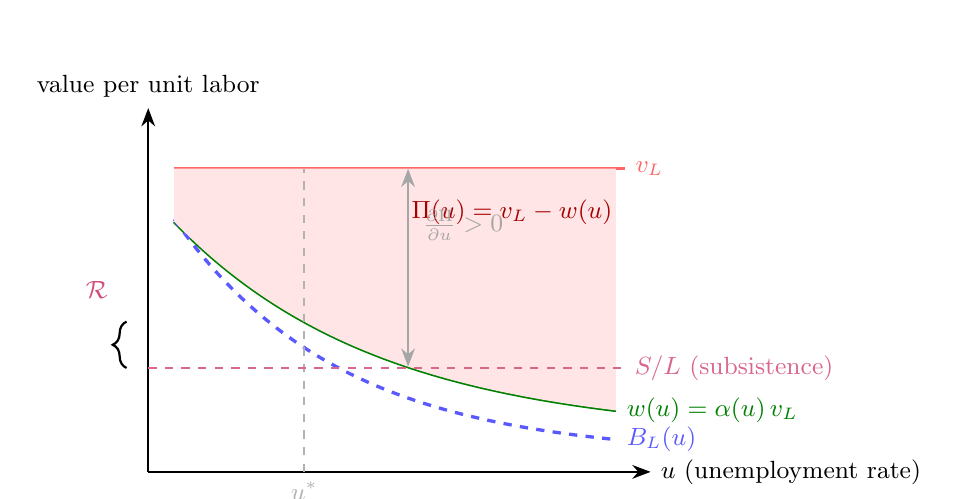
\begin{tikzpicture}[>=Stealth, thick, scale=1.1]
  \draw[->] (0,0) -- (5.8,0) node[right] {\small $u$ (unemployment rate)};
  \draw[->] (0,0) -- (0,4.2) node[above] {\small value per unit labor};

  % v_L constant
  \draw[red!60, very thick] (0.3, 3.5) -- (5.5, 3.5) node[right] {\small $v_L$};

  % alpha*v_L = W/L decreasing
  \draw[green!50!black, very thick] plot[smooth, domain=0.3:5.4, samples=60]
    (\x, {2.8*exp(-0.42*\x) + 0.42}) node[right] {\small $w(u) = \alpha(u)\,v_L$};

  % B_L decreasing
  \draw[blue!65, very thick, dashed] plot[smooth, domain=0.3:5.4, samples=60]
    (\x, {3.2*exp(-0.52*\x) + 0.18}) node[right] {\small $B_L(u)$};

  % Surplus shading
  \fill[red!10] plot[smooth, domain=0.3:5.4, samples=50]
    (\x, {2.8*exp(-0.42*\x)+0.42}) --
    (5.4, 3.5) -- (0.3, 3.5) -- cycle;
  \node[red!65!black, font=\small] at (4.2, 3.0) {$\Pi(u) = v_L - w(u)$};

  % Derivative annotation
  \draw[<->, gray!70] (3.0, {2.8*exp(-0.42*3)+0.42}) -- (3.0, 3.5);
  \node[gray!70, right, font=\small] at (3.05, 2.85) {$\frac{\partial\Pi}{\partial u}>0$};

  % Optimal u*
  \draw[dashed, gray!60] (1.8, 0) -- (1.8, 3.5);
  \node[below, gray!60, font=\small] at (1.8,0) {$u^*$};

  % Reproduction floor
  \draw[purple!60, dashed] (0, 1.2) -- (5.5, 1.2)
    node[right, font=\small, purple!60] {$S/L$ (subsistence)};

  % Bounded zone annotation
  \draw[decorate, decoration={brace, amplitude=5pt}]
    (-0.25, 1.2) -- (-0.25, {2.8*exp(-0.42*1.8)+0.42});
  \node[left, font=\small, purple!70] at (-0.35, 2.1) {$\mathcal{R}$};
\end{tikzpicture}
\caption{The unemployment gradient. Rising unemployment $u$ reduces bargaining power $B_L(u)$ (dashed blue), compressing the wage $w(u) = \alpha(u)\,v_L$ (green) and expanding the surplus $\Pi(u)$ (red shading). The bounded reproduction interval $\mathcal{R}$ lies between the subsistence floor $S/L$ and the full-value line $v_L$. The capital order manages $u$ to keep wages inside $\mathcal{R}$ while maximizing $\Pi$.}
\label{fig:unemployment}
\end{figure}

% ─────────────────────────────────────────────────
\section{Economic Theory as a Time-Indexed Projection Operator}
\label{sec:theory}

\subsection{The Possibility Space of Institutions}

Let $\Omega$ denote the full space of possible economic institutions---all conceivable arrangements of property rights, production organization, distribution mechanisms, and governance structures. $\Omega$ is a high-dimensional manifold. Its points include not only capitalist market configurations but cooperative economies, participatory planning systems, commons-based production, and indefinitely many hybrid forms.

Mattei argues that the function of neoclassical economics is to narrow the effective range of $\Omega$ considered within policy discourse. Mathematical models of rational agents, market equilibrium, and productive efficiency define a restricted subset from which policy proposals are drawn.

\begin{definition}[Time-Indexed Projection]
\label{def:projection}
Economic theory at time $t$ implements a projection operator
\begin{equation}
  \label{eq:projection}
  \mathcal{P}_t : \Omega \longrightarrow \Omega_t \;\subset\; \Omega,
\end{equation}
mapping the full institutional possibility space onto the historically specific subdomain $\Omega_t$ considered economically rational or feasible at $t$. The image $\Omega_t = \mathcal{P}_t(\Omega)$ evolves as the dominant economic paradigm shifts: it is larger during periods of theoretical pluralism (such as the 1930s debates over planning) and smaller during periods of neoclassical hegemony. Formally,
\begin{equation}
  \mathcal{P}_{t+1}(\Omega) \;\subseteq\; \Omega \quad\text{but}\quad
  \bigl|\Omega_{t+1}\bigr| \text{ varies with institutional history.}
\end{equation}
\end{definition}

The time-index is essential to Mattei's historical argument. She does not claim that the informational compression of neoclassical economics is eternal; she traces its historical construction through specific institutional interventions---the professionalization of economics, the marginalist revolution, the rise of central bank independence---that progressively narrowed $\Omega_t$. The projection operator is therefore itself a component of $I_t$ in the state vector $\mathcal{C}_t$, and changes in $\mathcal{P}_t$ correspond to ideological transformations within $I_t$.

\begin{definition}[Naturalization as Fixed-Point Claim]
Naturalization of the capital order corresponds to the false assertion that the attractor $\mathcal{A}_\mathcal{C}$ is the unique fixed point of $\Phi$ on all of $\Omega$:
\begin{equation}
  \Phi^n(\mathcal{C}_0) \to \mathcal{A}_\mathcal{C} \quad \forall\, \mathcal{C}_0 \in \Omega.
\end{equation}
This is precisely what neoclassical theory claims when it presents market equilibrium as universal. Mattei's historical argument refutes this by showing that $\mathcal{A}_\mathcal{C}$ is an attractor only within $\mathcal{B}(\mathcal{A}_\mathcal{C}) \subsetneq \mathcal{X}$, a basin maintained by political mechanisms rather than economic laws.
\end{definition}

\subsection{Semantic Entropy Reduction}

The operator $\mathcal{P}_t$ performs \emph{semantic entropy reduction} on the discourse manifold. By compressing the enormous complexity of social institutions into simplified mathematical representations---equilibrium curves, utility functions, production functions---it reduces the effective dimensionality of economic thought. In information-geometric terms, $\mathcal{P}_t$ decreases the volume of the admissible region:
\begin{equation}
  \mathrm{vol}(\Omega_t) \;<\; \mathrm{vol}(\Omega).
\end{equation}
When policy-makers, journalists, and citizens internalize the models encoded in $\mathcal{P}_t$, alternative economic arrangements appear not merely difficult to implement but literally unthinkable---they have been projected out of the conceptual manifold.

\begin{figure}[ht]
\centering
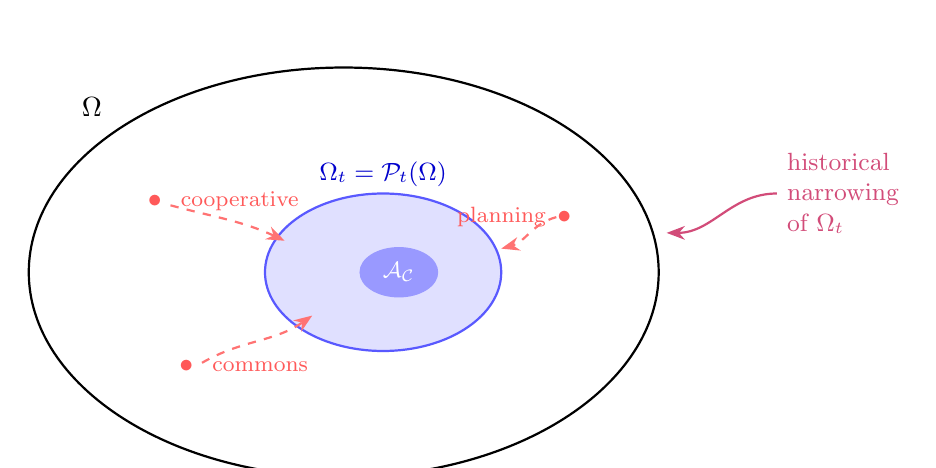
\begin{tikzpicture}[>=Stealth, thick]
  % Full Omega
  \draw[thick] (0,0) ellipse (4.0cm and 2.6cm);
  \node at (-3.2, 2.1) {$\Omega$};

  % Omega_t inside
  \fill[blue!12] (0.5, 0) ellipse (1.5cm and 1.0cm);
  \draw[blue!65, thick] (0.5, 0) ellipse (1.5cm and 1.0cm);
  \node[blue!80!black, font=\small] at (0.5, 1.25) {$\Omega_t = \mathcal{P}_t(\Omega)$};

  % Attractor inside Omega_t
  \fill[blue!40] (0.7, 0) ellipse (0.5cm and 0.32cm);
  \node[white, font=\footnotesize\bfseries] at (0.7, 0) {$\mathcal{A}_\mathcal{C}$};

  % Alternative institutions outside Omega_t
  \node[red!65, font=\normalsize] at (-2.4, 0.9) {$\bullet$};
  \node[red!65, font=\footnotesize, right] at (-2.2, 0.9) {cooperative};
  \node[red!65, font=\normalsize] at (-2.0, -1.2) {$\bullet$};
  \node[red!65, font=\footnotesize, right] at (-1.8,-1.2) {commons};
  \node[red!65, font=\normalsize] at (2.8, 0.7) {$\bullet$};
  \node[red!65, font=\footnotesize, left] at (2.7, 0.7) {planning};

  % Projection arrows
  \draw[->, red!55, dashed, thick] (-2.2, 0.85) to[out=-15, in=155] (-0.75, 0.4);
  \draw[->, red!55, dashed, thick] (-1.8,-1.15) to[out=30, in=215] (-0.4, -0.55);
  \draw[->, red!55, dashed, thick] (2.7, 0.7) to[out=195, in=15] (2.0, 0.3);

  % Historical evolution arrow
  \draw[->, thick, purple!70] (5.5, 1.0) to[out=180, in=0] (4.1, 0.5);
  \node[purple!70, right, font=\small, align=left] at (5.5, 1.0) {historical\\narrowing\\of $\Omega_t$};
\end{tikzpicture}
\caption{The time-indexed projection $\mathcal{P}_t$ collapses the full institutional possibility space $\Omega$ onto $\Omega_t$. Alternative configurations (cooperative ownership, commons, planning) are points of $\Omega$ but fall outside $\Omega_t$ and are thus excluded from legitimate economic discourse. The image $\Omega_t$ shrinks historically as neoclassical hegemony consolidates (purple arrow). The attractor $\mathcal{A}_\mathcal{C}$ lies at the center of $\Omega_t$ and is naturalized as the unique rational equilibrium.}
\label{fig:projection}
\end{figure}

% ─────────────────────────────────────────────────
\section{Technocracy as a Feedback Controller}
\label{sec:technocracy}

\subsection{The Macroeconomic State and the Controller}

Mattei's critique of technocracy identifies a functional governance layer that intermediates between democratic political pressure and economic outcomes. Central banks, fiscal authorities, international financial institutions, and academic economics departments function as observers of macroeconomic conditions who apply interventions to maintain the stability of the capital order. In control-theoretic terms, they constitute a \emph{feedback controller} for the institutional dynamical system.

Let the observable macroeconomic state be:
\begin{equation}
  X_t = \bigl(u(t),\; \pi(t),\; g(t),\; r(t),\; B_L(t)\bigr) \in \mathbb{R}^5,
\end{equation}
where $u$ is unemployment, $\pi$ inflation, $g$ growth, $r$ interest rates, and $B_L$ labor bargaining power. The policy component $P_t$ of the state vector $\mathcal{C}_t$ is determined by the feedback controller:
\begin{equation}
  \label{eq:controller}
  P_t = \Gamma(X_t),
\end{equation}
where $\Gamma : \mathbb{R}^5 \to \mathcal{P}$ maps observed macrostates to policy interventions. The design objective of $\Gamma$ is to minimize deviations of $\mathcal{C}_t$ from the surplus stability region $\mathcal{S}$:
\begin{equation}
  \label{eq:control_objective}
  \Gamma = \argmin_{P \in \mathcal{P}} \; d\!\bigl(\mathcal{C}_t(P),\; \mathcal{S}\bigr).
\end{equation}

\subsection{Technocracy as Curvature Regulation}

In RSVP terms, the controller $\Gamma$ regulates the curvature of the economic manifold. Interest rate decisions adjust the tension between investment and consumption gradients; fiscal rules define the permissible range of public resource allocation; employment targets constrain the acceptable range for $u(t)$. Together these instruments define the effective geometry of the field within which economic activity occurs.

The authority of technocratic institutions depends crucially on their claim to neutrality---the assertion that $\Gamma$ is not a political choice but a technical necessity dictated by economic law. Formally, this claim amounts to asserting that $\Gamma = \Gamma^*$, where $\Gamma^*$ is the uniquely correct policy function prescribed by economic theory. Mattei's critique is that $\Gamma^*$ is not derived from neutral principles but encodes the surplus stability region $\mathcal{S}$ as a design objective. The controller is not neutral; it is calibrated to reproduce the capital order.

\begin{figure}[ht]
\centering
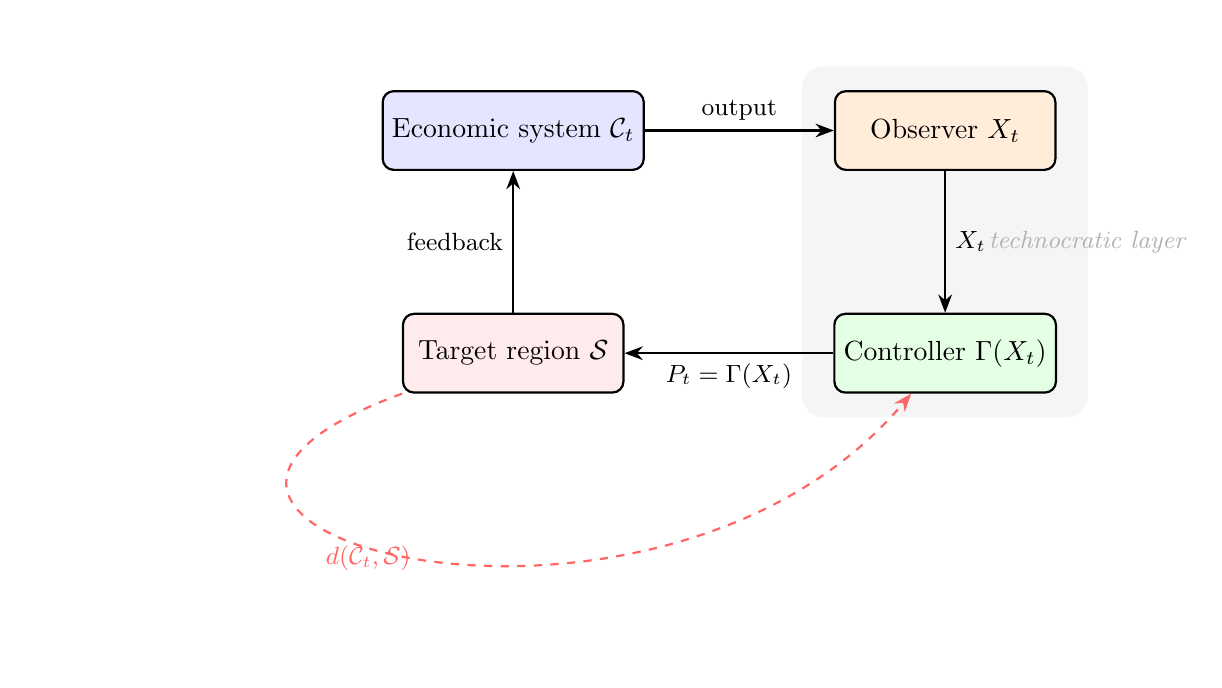
\begin{tikzpicture}[>=Stealth, thick, node distance=1.8cm]
  % Boxes
  \node[draw, rounded corners, minimum width=2.8cm, minimum height=1.0cm,
        fill=blue!10] (sys) {Economic system $\mathcal{C}_t$};
  \node[draw, rounded corners, minimum width=2.8cm, minimum height=1.0cm,
        fill=orange!15, right=2.4cm of sys] (obs) {Observer $X_t$};
  \node[draw, rounded corners, minimum width=2.8cm, minimum height=1.0cm,
        fill=green!10, below=1.8cm of obs] (ctrl) {Controller $\Gamma(X_t)$};
  \node[draw, rounded corners, minimum width=2.8cm, minimum height=1.0cm,
        fill=red!8, below=1.8cm of sys] (target) {Target region $\mathcal{S}$};

  % Arrows
  \draw[->] (sys) -- node[above, font=\small] {output} (obs);
  \draw[->] (obs) -- node[right, font=\small] {$X_t$} (ctrl);
  \draw[->] (ctrl) -- node[below, font=\small] {$P_t = \Gamma(X_t)$} (target);
  \draw[->] (target) -- node[left, font=\small] {feedback} (sys);

  % Error signal
  \draw[->, dashed, red!60] (target) to[out=200, in=230, looseness=2.0]
    node[left, font=\small, red!60] {$d(\mathcal{C}_t, \mathcal{S})$} (ctrl);

  % Label for technocratic layer
  \begin{scope}[on background layer]
    \fill[gray!8, rounded corners=8pt]
      ($(ctrl.south west)+(-0.4,-0.3)$) rectangle ($(obs.north east)+(0.4,0.3)$);
  \end{scope}
  \node[gray!60, font=\small\itshape] at ($(obs)!0.5!(ctrl)+(1.8,0)$) {technocratic layer};
\end{tikzpicture}
\caption{Technocracy as a feedback control architecture. The economic system produces observable macrostates $X_t$; the technocratic layer (shaded) maps these observations through the controller $\Gamma$ to generate policy interventions $P_t = \Gamma(X_t)$ designed to minimize deviations $d(\mathcal{C}_t, \mathcal{S})$ from the surplus stability region. The loop operates continuously, correcting perturbations before they can exit the basin of attraction.}
\label{fig:control}
\end{figure}

% ─────────────────────────────────────────────────
\section{Austerity as Stabilizing Feedback}
\label{sec:austerity}

\subsection{The Disciplinary Chain}

Mattei identifies austerity---cuts in public spending, wage suppression, monetary tightening---not as a neutral fiscal response to economic constraint but as a deliberate political intervention that restores the gradient structure of the capital order when democratic pressure has disturbed it. In dynamical terms, austerity functions as the primary corrective mechanism within $\Phi$: it provides the feedback signal that dampens oscillations threatening the attractor.

The formal content of this claim is expressed through the gradient chain derived in Section~\ref{sec:class}. Combining relations~\eqref{eq:bl_u}, \eqref{eq:pi_bl}, and~\eqref{eq:gradient_chain}:
\begin{equation}
  \label{eq:austerity_chain}
  u(t) \uparrow \;\Rightarrow\; B_L(t) \downarrow \;\Rightarrow\; \Pi(t) \uparrow,
\end{equation}
which formally expresses the austerity mechanism: raising unemployment reduces bargaining power, which compresses wages, which expands the surplus. The key insight is that unemployment is not a passive outcome of market forces but an \emph{active component} of the stabilizing feedback cycle embedded in $\Gamma$.

\subsection{Differential Equation of Correction}

The corrective dynamics of the bargaining power variable can be represented as:
\begin{equation}
  \label{eq:bl_ode}
  \frac{dB_L}{dt} = -\lambda\bigl(B_L(t) - B_L^*\bigr),
\end{equation}
where $B_L^* > 0$ is the target bargaining level consistent with the surplus stability condition $w < v_L$, and $\lambda > 0$ is the rate of correction implemented through austerity policy. The solution is exponential convergence:
\begin{equation}
  B_L(t) = B_L^* + \bigl(B_L(0) - B_L^*\bigr)\,e^{-\lambda t},
\end{equation}
representing the damped return of bargaining power toward the level at which the capital attractor is maintained. Stronger austerity corresponds to larger $\lambda$.

\subsection{Public Expenditure as Energy Injection}

In RSVP terms, public spending functions as an \emph{energy injection} into the social field: it finances welfare institutions, public employment, and collective consumption, increasing the effective autonomy of workers relative to market dependence and thereby weakening the survival coupling~\eqref{eq:individual_survival}. Let $E_{\mathrm{pub}}(t)$ denote this energy injection. Austerity is the operation:
\begin{equation}
  \frac{dE_{\mathrm{pub}}}{dt} < 0,
\end{equation}
which tightens the survival constraint, reduces $B_L$, and restores the gradient $v_L - w > 0$ required for accumulation. The higher the amplitude of the democratic perturbation, the larger the reduction in $E_{\mathrm{pub}}$ required to return $\mathcal{C}_t$ to $\mathcal{A}_\mathcal{C}$.

\begin{figure}[ht]
\centering
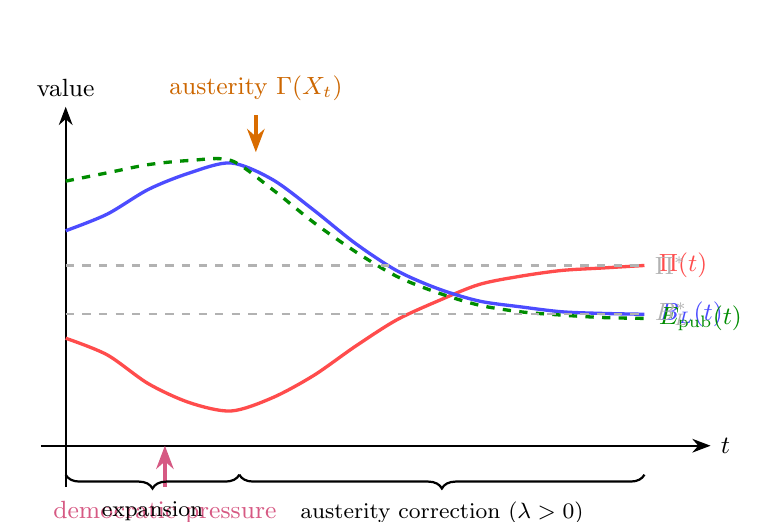
\begin{tikzpicture}[>=Stealth, thick, scale=1.05]
  \draw[->] (-0.3,0) -- (7.8,0) node[right] {\small $t$};
  \draw[->] (0,-0.5) -- (0,4.1) node[above] {\small value};

  % Surplus Pi
  \draw[red!70, very thick] plot[smooth] coordinates {
    (0,1.3)(0.5,1.1)(1.0,0.75)(1.5,0.52)(2.0,0.42)(2.5,0.58)
    (3.0,0.85)(3.5,1.2)(4.0,1.52)(4.5,1.75)(5.0,1.95)(5.5,2.05)
    (6.0,2.12)(6.5,2.15)(7.0,2.18)};
  \node[red!70, right] at (7.05, 2.18) {\small $\Pi(t)$};

  % Bargaining power B_L
  \draw[blue!70, very thick] plot[smooth] coordinates {
    (0,2.6)(0.5,2.8)(1.0,3.1)(1.5,3.3)(2.0,3.42)(2.5,3.22)
    (3.0,2.85)(3.5,2.45)(4.0,2.12)(4.5,1.9)(5.0,1.75)(5.5,1.68)
    (6.0,1.62)(6.5,1.60)(7.0,1.59)};
  \node[blue!70, right] at (7.05, 1.59) {\small $B_L(t)$};

  % E_pub
  \draw[green!55!black, very thick, dashed] plot[smooth] coordinates {
    (0,3.2)(0.5,3.3)(1.0,3.4)(1.5,3.45)(2.0,3.45)(2.5,3.1)
    (3.0,2.7)(3.5,2.35)(4.0,2.05)(4.5,1.85)(5.0,1.70)(5.5,1.62)
    (6.0,1.58)(6.5,1.55)(7.0,1.54)};
  \node[green!55!black, right] at (7.05, 1.54) {\small $E_{\mathrm{pub}}(t)$};

  % Target levels
  \draw[dashed, gray!60] (0, 2.18) -- (7.0, 2.18) node[right, gray!60] {\small $\Pi^*$};
  \draw[dashed, gray!60] (0, 1.59) -- (7.0, 1.59) node[right, gray!60] {\small $B_L^*$};

  % Austerity intervention
  \draw[orange!85!black, very thick, ->] (2.3, 4.0) -- (2.3, 3.55);
  \node[orange!80!black, above, font=\small] at (2.3, 4.05) {austerity $\Gamma(X_t)$};

  % Democratic pressure
  \draw[purple!65, very thick, ->] (1.2, -0.5) -- (1.2, 0.0);
  \node[purple!65, below, font=\small] at (1.2,-0.55) {democratic pressure};

  % Phase braces
  \draw[decorate, decoration={brace, mirror, amplitude=5pt}] (0,-0.35) -- (2.1,-0.35);
  \node[below, font=\footnotesize] at (1.05,-0.55) {expansion};
  \draw[decorate, decoration={brace, mirror, amplitude=5pt}] (2.1,-0.35) -- (7.0,-0.35);
  \node[below, font=\footnotesize] at (4.55,-0.55) {austerity correction ($\lambda > 0$)};
\end{tikzpicture}
\caption{The austerity stabilization cycle. Democratic pressure (purple) raises $B_L$ and compresses $\Pi$ during the expansion phase. Austerity (orange) is deployed by the controller $\Gamma(X_t)$, simultaneously withdrawing public energy $E_{\mathrm{pub}}$ (green dashed) and inducing unemployment, causing exponential convergence of $B_L \to B_L^*$ and $\Pi \to \Pi^*$ at rate $\lambda$.}
\label{fig:austerity}
\end{figure}

% ─────────────────────────────────────────────────
\section{The Institutional Potential Landscape}
\label{sec:potential}

\subsection{Austerity as a Democratic Constraint Mechanism}

The dominant public justification for austerity frames it as a technical remedy for fiscal imbalance: governments have overspent, structural deficits have accumulated, and corrective contraction is the prescription of responsible economic management. The formal framework developed in this paper offers a different interpretation. Austerity is not the response to fiscal deviation; it is the response to democratic deviation. It is deployed when democratic political pressures have moved the institutional trajectory toward the boundary of the surplus stability region $\mathcal{S}$, and its function is to return that trajectory to the interior of the capital attractor's basin.

A useful heuristic for making this structural function visible is the analogy of an institutional potential landscape. Imagine the policy space as a physical surface whose topography is determined by the institutional dynamical system. The capital order's attractor $\mathcal{A}_\mathcal{C}$ corresponds to a valley in this landscape: a region of minimum institutional potential to which trajectories are drawn by the dynamics of $\Phi$. Configurations farther from $\mathcal{A}_\mathcal{C}$---higher wages, expanded social provision, democratic control of investment---correspond to higher elevations in the potential landscape. They require continuous political energy to maintain against the restoring force of the capital order's corrective mechanisms.

Democratic pressures are forces that push the system uphill in this landscape. Austerity policies are the institutional analogue of gravity: the restoring force that returns displaced trajectories toward the valley.

\subsection{The Institutional Potential Function}

This analogy can be given formal content. Let $x \in \mathbb{R}^n$ parameterize the position of the institutional trajectory in policy space, with $x = 0$ corresponding to the capital attractor $\mathcal{A}_\mathcal{C}$. Define an institutional potential function $V : \mathbb{R}^n \to \mathbb{R}_{\geq 0}$ satisfying:
\begin{equation}
  \label{eq:potential}
  V(x) = 0 \iff x \in \mathcal{A}_\mathcal{C}, \qquad V(x) > 0 \;\text{ for }\; x \notin \mathcal{A}_\mathcal{C}.
\end{equation}
The institutional dynamics under the corrective action of $\Phi$ satisfy:
\begin{equation}
  \label{eq:potential_decrease}
  \frac{dV}{dt} = \nabla V \cdot \dot{x} \leq 0,
\end{equation}
with equality only at $\mathcal{A}_\mathcal{C}$. In dynamical systems terminology, $V$ is a Lyapunov function for the capital attractor: it decreases along all trajectories within the basin $\mathcal{B}(\mathcal{A}_\mathcal{C})$, confirming that $\mathcal{A}_\mathcal{C}$ is asymptotically stable under the institutional dynamics.

\begin{definition}[Institutional Potential]
A function $V : \mathcal{X} \to \mathbb{R}_{\geq 0}$ is an institutional potential for the capital order if it satisfies~\eqref{eq:potential} and~\eqref{eq:potential_decrease} on $\mathcal{B}(\mathcal{A}_\mathcal{C})$. In the scalar single-dimensional case, a natural choice is
\begin{equation}
  \label{eq:quadratic_potential}
  V(x) = \frac{1}{2}\,k\,x^2,
\end{equation}
where $k > 0$ measures the stiffness of the institutional restoring force---the rate at which corrective pressures increase as the trajectory deviates from $\mathcal{A}_\mathcal{C}$. A higher $k$ corresponds to a steeper valley and a more aggressive corrective response per unit deviation.
\end{definition}

The austerity correction rate $\lambda$ introduced in equation~\eqref{eq:bl_ode} is directly related to $k$: the exponential convergence $B_L(t) \to B_L^*$ at rate $\lambda$ corresponds to the gradient descent $\dot x = -\lambda\, \nabla V(x)$ along the potential surface. Austerity increases $\lambda$, thereby steepening $V$ and accelerating the return to the attractor.

\subsection{Democratic Pressure and Potential Energy}

Democratic political pressure that pushes wages toward $v_L$, expands public spending, or strengthens labor bargaining power can be modeled as a force $F_{\text{dem}}(t)$ applied to the system that increases the potential energy of the institutional configuration:
\begin{equation}
  \frac{dV}{dt} = \nabla V \cdot \dot x = -\lambda V + F_{\text{dem}}(t).
\end{equation}
The institutional trajectory moves away from $\mathcal{A}_\mathcal{C}$ when $F_{\text{dem}}(t) > \lambda V(x(t))$---when the democratic force exceeds the restoring force of the capital order. Austerity increases $\lambda$; it raises the threshold that democratic forces must exceed to displace the system from its attractor. This is the formal content of the claim that austerity constrains democratic space: it does not directly prevent democratic political activity, but it increases the institutional energy required to maintain any democratic deviation from the capital attractor.

\subsection{Constraining Democratic Dimensionality}

Austerity's effect on the policy manifold dimension $D$ introduced in Section~\ref{sec:authoritarianism} can now be interpreted in potential-landscape terms. High-$D$ democratic governance implies a rugged potential landscape with local variations: different policy trajectories are possible, and the system can explore a range of configurations within and near $\mathcal{B}(\mathcal{A}_\mathcal{C})$. Austerity smooths this landscape---it reduces the local curvature of $V$ in directions corresponding to democratic policy variation, making it energetically costly to maintain any configuration away from $\mathcal{A}_\mathcal{C}$. Formally:
\begin{equation}
  \text{Hess}(V)\big|_{\text{under austerity}} \;\succ\; \text{Hess}(V)\big|_{\text{without austerity}},
\end{equation}
meaning the Hessian of the potential under austerity is larger (in the positive-definite sense) than under democratic governance. The valley is steeper, the restoring force stronger, and the effective policy space available to democratic institutions narrower.

\begin{remark}
The potential-landscape interpretation connects directly to the RSVP framework. In RSVP terms, $V(x)$ measures the degree to which the institutional configuration departs from the non-equilibrium steady state that sustains the capital order. The gradient $\nabla V$ is the RSVP flux field $\mathbf{v}$ directed toward $\mathcal{A}_\mathcal{C}$. Austerity increases the magnitude of $\mathbf{v}$ in the direction of the attractor, counteracting the democratic forces that would flatten the gradient $\nabla(\varrho_K - \varrho_L)$.
\end{remark}

\subsection{One-Dimensional Potential Landscape}

\begin{figure}[ht]
\centering
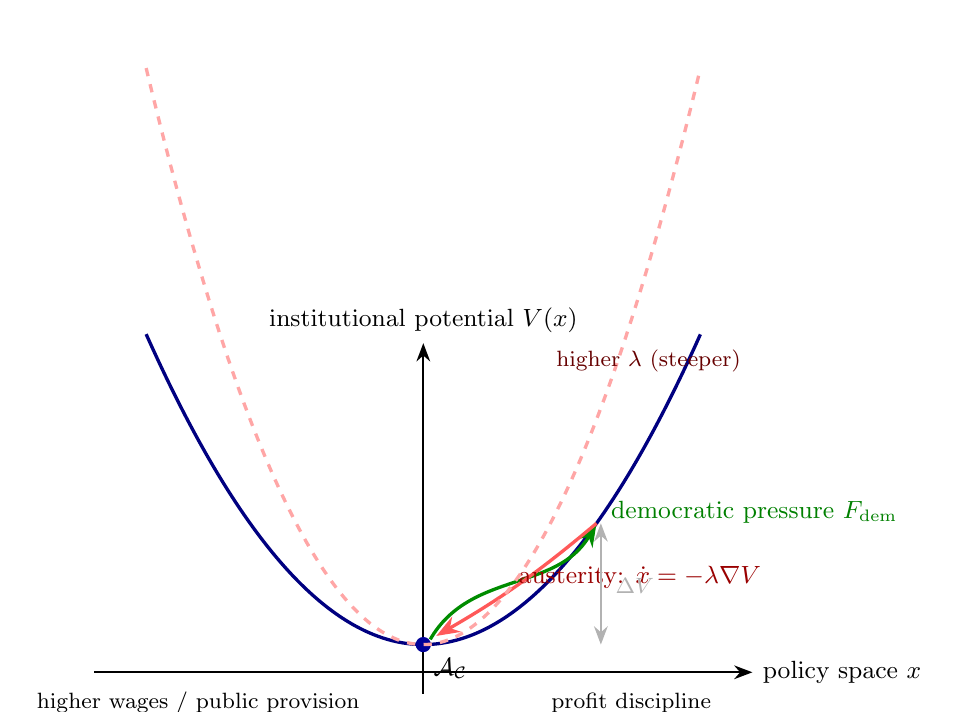
\begin{tikzpicture}[>=Stealth, thick, scale=1.1]
  % Axes
  \draw[->] (-3.8,0) -- (3.8,0)
    node[right, font=\small] {policy space $x$};
  \draw[->] (0,-0.25) -- (0,3.8)
    node[above, font=\small] {institutional potential $V(x)$};

  % Valley curve V = 0.35 x^2 + 0.32
  \draw[very thick, blue!50!black]
    plot[smooth, domain=-3.2:3.2, samples=120]
    (\x, {0.35*\x*\x + 0.32});

  % Attractor point
  \fill[blue!60!black] (0, 0.32) circle (2.5pt);
  \node[below right, font=\small] at (0, 0.28) {$\mathcal{A}_\mathcal{C}$};

  % Democratic push: arrow from attractor up-right
  \draw[->, very thick, green!55!black]
    (0.08, 0.38) to[out=60, in=240] (2.0, 1.72);
  \node[green!50!black, font=\small, right] at (2.05, 1.85)
    {democratic pressure $F_{\text{dem}}$};

  % Austerity restoring: arrow back down to attractor
  \draw[->, very thick, red!65]
    (2.0, 1.72) to[out=220, in=30] (0.15, 0.42);
  \node[red!60!black, font=\small] at (2.5, 1.1)
    {austerity: $\dot x = -\lambda \nabla V$};

  % Higher-lambda steeper curve
  \draw[very thick, red!35, dashed]
    plot[smooth, domain=-3.2:3.2, samples=120]
    (\x, {0.65*\x*\x + 0.32});
  \node[red!40!black, font=\footnotesize] at (2.6, 3.6)
    {higher $\lambda$ (steeper)};

  % Axis labels
  \node[font=\footnotesize] at (-2.6, -0.35) {higher wages / public provision};
  \node[font=\footnotesize] at (2.4, -0.35) {profit discipline};

  % Energy annotation
  \draw[<->, gray!60] (2.05, 0.32) -- (2.05, 1.72);
  \node[gray!60, font=\footnotesize, right] at (2.1, 1.0) {$\Delta V$};
\end{tikzpicture}
\caption{One-dimensional institutional potential landscape $V(x) = \tfrac{1}{2}kx^2$. The attractor $\mathcal{A}_\mathcal{C}$ corresponds to the valley minimum. Democratic pressure (green arrow) increases the potential energy of the configuration by $\Delta V$. Austerity (red arrow) implements gradient descent $\dot x = -\lambda \nabla V$, returning the trajectory to the attractor. The dashed curve shows the steeper potential under higher austerity rate $\lambda$, narrowing the effective policy space available to democratic intervention.}
\label{fig:valley_1d}
\end{figure}

\subsection{Two-Dimensional Contour Basin}

The one-dimensional representation simplifies policy space to a single axis. A more informative picture is obtained in two dimensions, where the policy space is parameterized by wage share and democratic policy autonomy.

\begin{figure}[ht]
\centering
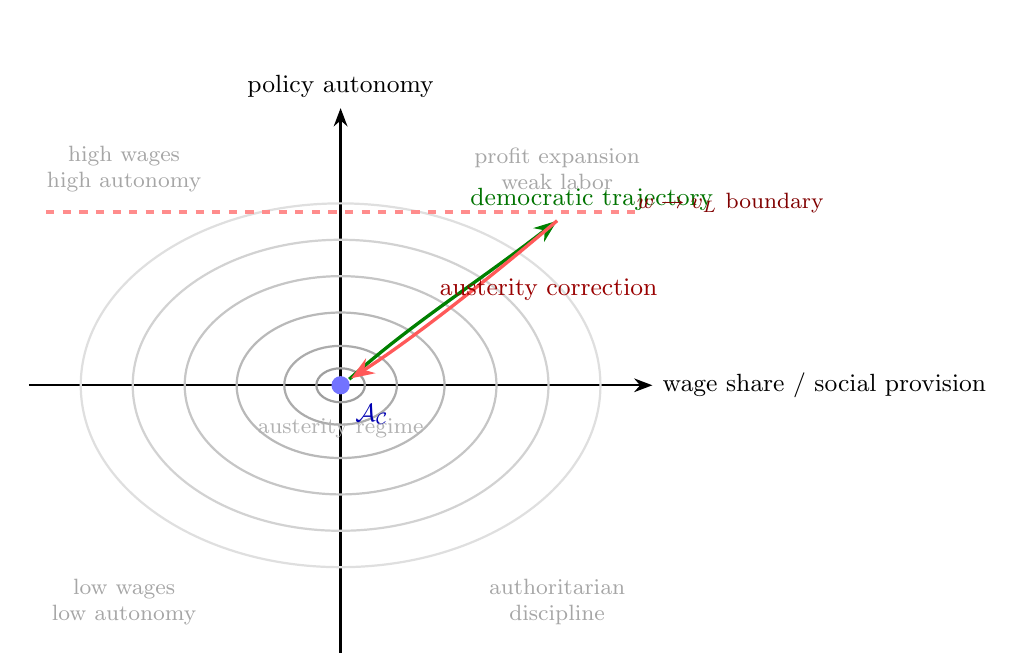
\begin{tikzpicture}[>=Stealth, thick, scale=1.1]
  % Axes
  \draw[->] (-3.6,0) -- (3.6,0)
    node[right, font=\small] {wage share / social provision};
  \draw[->] (0,-3.2) -- (0,3.2)
    node[above, font=\small] {policy autonomy};

  % Contour ellipses (level sets of V)
  \foreach \a/\b/\col in {
    3.0/2.1/gray!25,
    2.4/1.68/gray!35,
    1.8/1.26/gray!45,
    1.2/0.84/gray!55,
    0.65/0.455/gray!65,
    0.28/0.196/gray!75
  }{
    \draw[\col, thick] (0,0) ellipse (\a cm and \b cm);
  }

  % Attractor at center
  \fill[blue!55] (0,0) circle (3pt);
  \node[below right, font=\small, blue!70!black] at (0.05,-0.1) {$\mathcal{A}_\mathcal{C}$};

  % Neoliberal / austerity label inside basin
  \node[font=\footnotesize, gray!60] at (0, -0.5) {austerity regime};

  % Democratic trajectory (blue curve)
  \draw[->, very thick, green!50!black]
    (0.1, 0.07) .. controls (0.8, 0.7) and (1.6, 1.2) .. (2.5, 1.9);
  \node[green!45!black, font=\small] at (2.9, 2.15)
    {democratic trajectory};

  % Austerity correction (red curve)
  \draw[->, very thick, red!65]
    (2.5, 1.9) .. controls (1.5, 1.05) and (0.7, 0.45) .. (0.12, 0.08);
  \node[red!60!black, font=\small] at (2.4, 1.1)
    {austerity correction};

  % Quadrant labels
  \node[font=\footnotesize, align=center, gray!70] at (-2.5, 2.5)
    {high wages\\high autonomy};
  \node[font=\footnotesize, align=center, gray!70] at (2.5, 2.5)
    {profit expansion\\weak labor};
  \node[font=\footnotesize, align=center, gray!70] at (-2.5,-2.5)
    {low wages\\low autonomy};
  \node[font=\footnotesize, align=center, gray!70] at (2.5,-2.5)
    {authoritarian\\discipline};

  % Surplus stability boundary annotation
  \draw[red!45, very thick, dashed] (-3.4, 2.0) -- (3.4, 2.0);
  \node[red!50!black, font=\footnotesize, right] at (3.3, 2.1)
    {$w \to v_L$ boundary};
\end{tikzpicture}
\caption{Two-dimensional institutional potential basin. Level curves (contours of $V(x,y)$) represent the restoring force of the capital order. The democratic trajectory (green) moves the system outward toward higher wage shares and greater policy autonomy. Austerity (red curve) redirects the trajectory back toward $\mathcal{A}_\mathcal{C}$. The dashed line marks the boundary $w \to v_L$ at which the surplus stability condition begins to fail. Configurations above this boundary represent the effective outer limit of the democratic challenge that the capital order must counteract.}
\label{fig:basin_2d}
\end{figure}

\subsection{Three-Dimensional Potential Surface}

The three-dimensional rendering below gives the potential landscape its fullest geometric expression, making the valley structure and the two competing forces simultaneously visible as a surface embedded in policy-potential space.

\begin{figure}[ht]
\centering
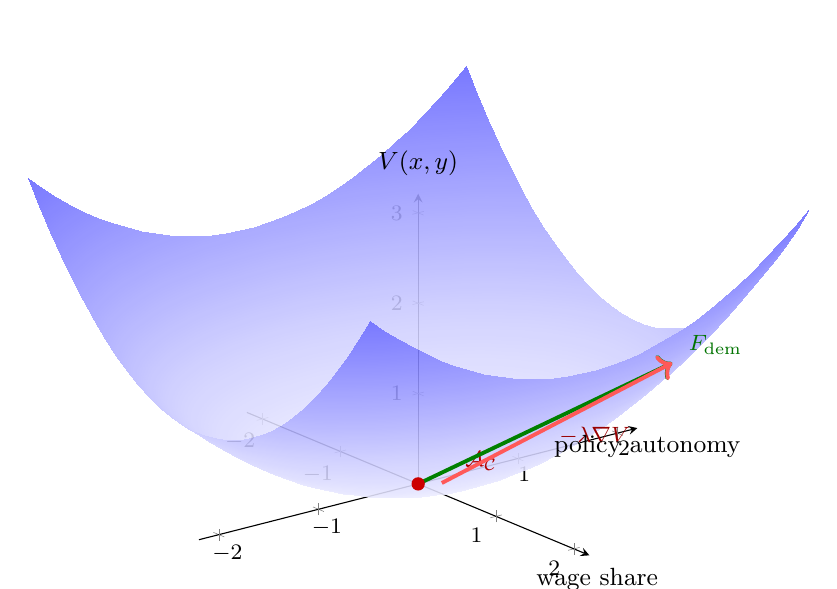
\begin{tikzpicture}
\begin{axis}[
    view={52}{32},
    axis lines=center,
    xlabel={\small wage share},
    ylabel={\small policy autonomy},
    zlabel={\small $V(x,y)$},
    xlabel style={at={(axis cs:2.3,0,0)}, anchor=north},
    ylabel style={at={(axis cs:0,2.3,0)}, anchor=north},
    zlabel style={at={(axis cs:0,0,3.3)}, anchor=south},
    domain=-2.2:2.2,
    domain y=-2.2:2.2,
    samples=32,
    colormap={bluevalley}{
      color=(blue!5) color=(blue!20) color=(blue!40) color=(blue!60)},
    width=11.5cm,
    height=8.5cm,
    z buffer=sort,
    xtick={-2,-1,0,1,2},
    ytick={-2,-1,0,1,2},
    ztick={0,1,2,3,4},
    tick label style={font=\footnotesize},
    clip=false
]
  % Potential surface V = 0.4(x^2 + 0.6 y^2)
  \addplot3[surf, opacity=0.88, shader=interp]
    {0.42*(x^2 + 0.58*y^2)};

  % Attractor point at minimum
  \addplot3[only marks, mark=*, mark size=2.2pt, color=red!80!black]
    coordinates {(0,0,0)};
  \node[font=\footnotesize, red!70!black] at (axis cs:0.3,0.4,0.25)
    {$\mathcal{A}_\mathcal{C}$};

  % Democratic pressure vector
  \addplot3[->, very thick, color=green!50!black, line width=1.4pt]
    coordinates {(0,0,0) (1.6,1.3,1.55)};
  \node[font=\footnotesize, green!45!black] at (axis cs:1.9,1.5,1.8)
    {$F_{\text{dem}}$};

  % Austerity restoring vector
  \addplot3[->, very thick, color=red!65, line width=1.4pt]
    coordinates {(1.6,1.3,1.55) (0.15,0.12,0.03)};
  \node[font=\footnotesize, red!60!black] at (axis cs:1.5,0.6,0.9)
    {$-\lambda\nabla V$};

\end{axis}
\end{tikzpicture}
\caption{Three-dimensional institutional potential surface $V(x,y) = 0.42\,(x^2 + 0.58\,y^2)$ over the policy space parameterized by wage share ($x$-axis) and democratic policy autonomy ($y$-axis). The valley minimum corresponds to $\mathcal{A}_\mathcal{C}$. The green vector $F_{\text{dem}}$ represents democratic pressure increasing the system's potential energy by moving it away from the attractor. The red vector $-\lambda\nabla V$ represents the austerity-driven gradient descent that returns the system toward the minimum. Steeper austerity (larger $\lambda$) narrows the accessible policy space by increasing the energetic cost of maintaining configurations away from $\mathcal{A}_\mathcal{C}$.}
\label{fig:surface_3d}
\end{figure}

\subsection{Implications for Structural Transformation}

The potential-landscape framework clarifies two things simultaneously. First, it explains why isolated democratic policy victories are typically temporary: as long as the potential landscape retains the same topography---as long as the institutional dynamics of $\Phi$ continue to implement gradient descent toward $\mathcal{A}_\mathcal{C}$---any configuration displaced from the attractor will eventually be returned to it by the corrective mechanisms of the capital order. Social-democratic welfare states, for instance, correspond to sustained displacement from $\mathcal{A}_\mathcal{C}$ maintained against the restoring force by continuous political energy. When that political energy dissipates---as it did during the neoliberal turn of the 1970s and 1980s---the restoring force returns the system toward the attractor.

Second, it clarifies what structural transformation requires: not merely more political energy to displace the trajectory further uphill, but a change in the topography of the landscape itself. Transforming the capital order means altering the location or character of the attractor $\mathcal{A}_\mathcal{C}$, either by eliminating it entirely and replacing it with a different attractor $\mathcal{A}'$, or by flattening the potential surface so that the restoring force toward $\mathcal{A}_\mathcal{C}$ is weakened. This corresponds precisely to the constraint-redefinition analysis of Section~\ref{sec:democracy}: changing ownership structures, dissolving the survival coupling, or expanding the discourse manifold's curvature all alter the potential function $V$ rather than merely displacing the system within its existing landscape.

% ─────────────────────────────────────────────────
\section{Authoritarian Stabilization as Dimensionality Reduction}
\label{sec:authoritarianism}

\subsection{The Policy Manifold and its Dimension}

Mattei's historical analysis identifies a recurrent pattern: when democratic institutions introduce significant variability into economic governance, capitalist and technocratic actors have supported authoritarian solutions to restore economic discipline. We formalize this through the concept of the policy manifold.

Let $\mathcal{M}_D$ denote the policy manifold---the space of possible governance configurations accessible under the prevailing political system---with effective dimensionality $\dim(\mathcal{M}_D) = D$. Under robust democratic governance, $D$ is large: questions about ownership, investment, wages, public services, and fiscal architecture are all potentially open to collective political determination. High dimensionality implies that the trajectory $\mathcal{C}_t$ has access to a large region of $\mathcal{X}$, including regions outside $\mathcal{B}(\mathcal{A}_\mathcal{C})$.

\begin{proposition}[Authoritarian Dimensionality Reduction]
Authoritarian governance imposes constraints that restrict the accessible policy manifold to a lower-dimensional submanifold:
\begin{equation}
  \mathcal{M}_{\mathrm{auth}} \subset \mathcal{M}_D, \qquad
  \dim(\mathcal{M}_{\mathrm{auth}}) < D.
\end{equation}
This restriction prevents $\mathcal{C}_t$ from exploring trajectories that would exit $\mathcal{B}(\mathcal{A}_\mathcal{C})$, thereby stabilizing the capital attractor.
\end{proposition}

\begin{proof}[Sketch]
Democratic deliberation allows variation along $D$ independent policy dimensions. Authoritarian rule removes or freezes $k < D$ of these dimensions through suppression of labor organizations, abolition of parliamentary oversight, censorship of economic alternatives, and direct executive control of monetary and fiscal policy. The accessible manifold therefore reduces from $\mathcal{M}_D$ to a submanifold of dimension $D - k$, restricting the phase space available for democratic perturbation.
\end{proof}

\subsection{Lyapunov Dimension and Attractor Stability}

In dynamical systems terms, reducing the dimensionality of the accessible state space lowers the Lyapunov dimension of the system's accessible trajectories. Fewer degrees of freedom are available for perturbation, and the corrective force of $\Phi$ toward $\mathcal{A}_\mathcal{C}$ is stronger because deviations are constrained to a lower-dimensional subspace.

This formalizes the historical coherence that Mattei documents: the collaboration between economists and authoritarian regimes in the 1920s was not ideologically inconsistent but structurally complementary. Technocratic austerity and authoritarian politics are parallel stabilizing mechanisms operating at different levels of the system---one reducing economic gradients, the other reducing political degrees of freedom.

\begin{corollary}[Complementarity of Austerity and Authoritarianism]
Let $\lambda$ be the austerity correction rate in~\eqref{eq:bl_ode} and $D$ the democratic dimensionality of the policy manifold. The effective stability of $\mathcal{A}_\mathcal{C}$ is a joint function of both:
\begin{equation}
  \text{stability}(\mathcal{A}_\mathcal{C}) = h(\lambda, D^{-1}),
\end{equation}
where $h$ is increasing in $\lambda$ and in $D^{-1}$. Higher austerity rates and lower democratic dimensionality reinforce each other in sustaining the capital attractor.
\end{corollary}

% ─────────────────────────────────────────────────
\section{RSVP Translation of the Capital Order}
\label{sec:rsvp}

\subsection{The Plenum as Economic Field}

The Relativistic Scalar-Vector Plenum (RSVP) framework models complex systems as fields in which scalar entropy density $\varrho(x,t)$ and a vector smoothing flux $\mathbf{v}(x,t)$ interact across a manifold $\mathcal{M}$. The central dynamical principle is that structured systems persist by maintaining \emph{controlled asymmetries}---gradient differentials that drive flux while preventing equilibration.

The capital order is a RSVP subsystem embedded in the broader social plenum. Its structural features correspond to RSVP field-theoretic concepts as follows.

\subsection{Labor as Entropy Transduction Node}

Workers function as \emph{entropy transduction nodes}: biological energy requirements drive the conversion of metabolic potential into economic labor, sustaining the flow of value through the production field. The survival-coupling constraint~\eqref{eq:individual_survival} means that the coupling between individual thermodynamic necessity and systemic throughput is binding.

Let $\varrho_L(x,t)$ and $\varrho_K(x,t)$ denote labor-energy and capital-energy density fields respectively. The surplus extraction condition requires a persistent gradient:
\begin{equation}
  \nabla\!\bigl(\varrho_K - \varrho_L\bigr) > 0,
\end{equation}
directed from regions of labor activity toward capital accumulation structures. Institutions---firms, property law, financial systems---are channels that maintain this gradient by preventing spontaneous equilibration.

\subsection{The Capital Attractor as Non-Equilibrium Steady State}

In RSVP cosmology, structures persist when they reach configurations that minimize local entropy production while maintaining the global gradient differentials driving systemic throughput. The capital order represents such a configuration: it is not at thermodynamic equilibrium (which would require $\varrho_K = \varrho_L$) but at a \emph{non-equilibrium steady state} sustained by continuous institutional work. The RSVP evolution equation for entropy density is:
\begin{equation}
  \label{eq:rsvp_evolution}
  \partial_t \varrho + \nabla \cdot (\varrho\, \mathbf{v}) = \sigma,
\end{equation}
where $\mathbf{v}$ is the smoothing flux and $\sigma > 0$ is entropy production at the labor-capital interface---a persistent irreversibility maintained by the coupling constraints.

Austerity policies are \emph{anti-smoothing operations}: they steepen the gradient $\nabla(\varrho_K - \varrho_L)$ when it begins to flatten under democratic pressure, counteracting the natural smoothing dynamics of the RSVP field.

\subsection{Economic Theory as Semantic Smoothing Operator}

Let $\mathcal{S}_{\mathrm{disc}}$ denote the semantic manifold of economic discourse, with curvature tensor $\kappa(\mathcal{S}_{\mathrm{disc}})$. The time-indexed projection $\mathcal{P}_t$ reduces semantic curvature:
\begin{equation}
  \bigl\|\kappa\!\bigl(\mathcal{P}_t(\mathcal{S}_{\mathrm{disc}})\bigr)\bigr\| < \bigl\|\kappa(\mathcal{S}_{\mathrm{disc}})\bigr\|,
\end{equation}
flattening the landscape of institutional possibility. In a flat semantic manifold, all discursive paths appear to lead toward the same equilibrium---the capital attractor---because the curvature that would direct attention toward alternative configurations has been suppressed by the projection.

\begin{figure}[ht]
\centering
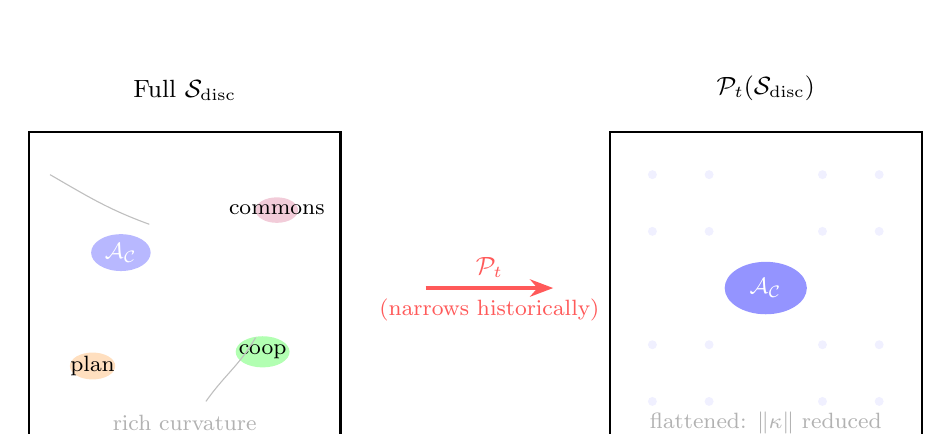
\begin{tikzpicture}[>=Stealth, thick, scale=0.9]
  % Full semantic landscape
  \begin{scope}[xshift=-4.2cm]
    \node[above, font=\small] at (0,2.5) {Full $\mathcal{S}_{\mathrm{disc}}$};
    \draw[thick] (-2.2,-2.2) rectangle (2.2,2.2);
    \fill[blue!28] (-0.9, 0.5) ellipse (0.42 and 0.26);
    \node[white, font=\footnotesize\bfseries] at (-0.9, 0.5) {$\mathcal{A}_\mathcal{C}$};
    \fill[green!30] (1.1, -0.9) ellipse (0.38 and 0.22);
    \node[font=\footnotesize] at (1.1,-0.9) {coop};
    \fill[orange!25] (-1.3, -1.1) ellipse (0.32 and 0.19);
    \node[font=\footnotesize] at (-1.3,-1.1) {plan};
    \fill[purple!20] (1.3, 1.1) ellipse (0.30 and 0.18);
    \node[font=\footnotesize] at (1.3, 1.1) {commons};
    \draw[gray!50, thin] (-1.9, 1.6) to[out=-30, in=160] (-0.5, 0.9);
    \draw[gray!50, thin] (0.3, -1.6) to[out=55, in=240] (1.0, -0.7);
    \node[gray!60, font=\footnotesize] at (0, -1.9) {rich curvature};
  \end{scope}

  % Projection arrow
  \draw[->, very thick, red!65] (-0.8, 0) -- (1.0, 0)
    node[midway, above, font=\small] {$\mathcal{P}_t$}
    node[midway, below, font=\footnotesize] {(narrows historically)};

  % Flattened manifold
  \begin{scope}[xshift=4.0cm]
    \node[above, font=\small] at (0,2.5) {$\mathcal{P}_t(\mathcal{S}_{\mathrm{disc}})$};
    \draw[thick] (-2.2,-2.2) rectangle (2.2,2.2);
    \fill[blue!42] (0, 0) ellipse (0.58 and 0.37);
    \node[white, font=\footnotesize\bfseries] at (0,0) {$\mathcal{A}_\mathcal{C}$};
    \foreach \x in {-1.6,-0.8,0.8,1.6} {
      \foreach \y in {-1.6,-0.8,0.8,1.6} {
        \fill[blue!6] (\x, \y) circle (1.8pt);
      }
    }
    \node[gray!60, font=\footnotesize] at (0,-1.9) {flattened: $\|\kappa\|$ reduced};
  \end{scope}
\end{tikzpicture}
\caption{Economic theory as semantic smoothing. The full discourse manifold $\mathcal{S}_{\mathrm{disc}}$ contains rich curvature with multiple viable attractors. The time-indexed projection $\mathcal{P}_t$ flattens the manifold, leaving only $\mathcal{A}_\mathcal{C}$ visible. The image shrinks historically as the neoclassical paradigm consolidates. Alternative institutions become unthinkable rather than merely impractical.}
\label{fig:semantic}
\end{figure}

% ─────────────────────────────────────────────────
\section{Toward a Democratic Economic Topology}
\label{sec:democracy}

\subsection{Constraint Redefinition as Attractor Shift}

Mattei's proposal for escaping capitalism is a call for the democratization of economic decision-making: a collective reclaiming of authority over institutional parameters. In the formal framework developed here, this corresponds not to a perturbation within the existing basin of attraction but to a \emph{redefinition of the constraint structure} that defines the surplus stability region $\mathcal{S}$.

The capital order is sustained by three interlocking constraints: the survival coupling~\eqref{eq:individual_survival}--\eqref{eq:collective_survival} forcing market participation; the surplus extraction condition $w < v_L$ ensuring value flow toward capital; and the projection $\mathcal{P}_t$ restricting deliberation to $\Omega_t$. Democratic transformation requires altering each. Consider the transformed state:
\begin{equation}
  \mathcal{C}_t' = \bigl(L_t,\, K_t',\, P_t',\, I_t'\bigr),
\end{equation}
where $K_t'$ includes cooperative or public ownership structures; $P_t'$ includes participatory governance that expands $D$; and $I_t'$ operates with a projection $\mathcal{P}_t'$ whose image $\Omega_t'$ is substantially larger than $\Omega_t$.

\subsection{Democratic Redefinition of the Stability Region}

The surplus extraction condition $w < v_L$ defines the stability region $\mathcal{S}$ for the capital order. Democratic transformation corresponds to replacing this stability target. In a cooperative system in which workers control production decisions, the distributional rule shifts toward:
\begin{equation}
  w \;\approx\; v_L \quad\Longleftrightarrow\quad \Pi \approx 0,
\end{equation}
or more generally toward a democratic allocation function:
\begin{equation}
  Y_t = D(L_t, K_t'),
\end{equation}
where $D$ represents collectively determined distributional rules rather than the privately appropriated residual of neoclassical profit. The stability region of the new system is:
\begin{equation}
  \mathcal{S}' = \bigl\{\,\mathcal{C}' : w \approx v_L,\quad D\text{ collectively determined}\,\bigr\},
\end{equation}
which is geometrically disjoint from $\mathcal{S}$: the two stability regions occupy different subsets of the institutional state space $\mathcal{X}$.

\subsection{Decoupling Survival from Capital}

The most fundamental transformation is the weakening of the survival coupling. Mechanisms such as universal public provisioning, cooperative production, or commons-based resource access modify the individual income equation:
\begin{equation}
  w_i(t) = f_i(L_i, M) + g_i\!\bigl(\text{public}, t\bigr),
\end{equation}
where $g_i > 0$ represents income derived from non-market institutional channels. As $g_i$ grows, the binding force of constraint~\eqref{eq:individual_survival} relaxes. The labor reproduction equation~\eqref{eq:labor_repro} becomes:
\begin{equation}
  L_{t+1} = R\!\bigl(L_t,\, W(t) + G(t),\, S(t)\bigr),
\end{equation}
where $G(t) = \sum_i g_i(t)$ is aggregate non-market provisioning. Sufficient $G(t)$ decouples labor reproduction from wage discipline, weakening the gradient $v_L - w$ that the capital order depends on.

\subsection{Gradient Redistribution in RSVP Terms}

In RSVP language, democratic transformation redistributes the gradients of energy, meaning, and agency within the social plenum. The persistent differential $\nabla(\varrho_K - \varrho_L) > 0$ is flattened---not by coercive equalization but by restructuring the institutional channels through which value flows. New attractor structures emerge in the social field as the energy density that previously concentrated in ownership structures is redistributed through collective institutions. The semantic manifold recovers curvature, restoring the landscape of institutional possibility that $\mathcal{P}_t$ had compressed.

This does not guarantee that a democratic configuration is stable or self-maintaining. Just as the capital order requires continuous institutional work to sustain its gradient structure, alternative configurations require the construction of new institutional channels, governance mechanisms, and cultural frameworks. The RSVP perspective clarifies that transformation is not a single event but an ongoing dynamical project---a continuous reorganization of the gradients that determine how value, energy, and meaning flow through the social system.

% ─────────────────────────────────────────────────
\section{Crisis Cycles and Systemic Reproduction}
\label{sec:crisis_cycles}

\subsection{Crisis as Structural Regularity}

Capitalism does not reproduce itself through a stable equilibrium. Its continuity depends on recurrent oscillations between phases of expansion and phases of disciplinary correction. Classical political economy already recognized this tendency: Marx described crises as moments when the contradictions of accumulation become unavoidably visible, while Hyman Minsky demonstrated that financial stability itself tends over time to generate the conditions for instability. Within the framework developed here, these dynamics are interpretable as the natural consequence of a system whose trajectory must be continuously maintained within a stability region through active feedback---a system that therefore oscillates cyclically rather than converging to rest.

The macroeconomic state vector $X_t = (u_t, \pi_t, r_t, g_t, \Pi_t)$ introduced in Section~\ref{sec:technocracy} evolves under the transition rule $X_{t+1} = F(X_t, P_t)$. During expansion phases, accumulation increases $g_t$ and $\Pi_t$ while employment rises, tightening labor markets and beginning to strengthen $B_L$. The surplus stability condition $w < v_L$ gradually tightens as wages respond to falling unemployment. This is the endogenous destabilization mechanism: the very success of accumulation generates the forces that will eventually compress it.

\subsection{The Goodwin Mechanism}

The most compact formal representation of this cyclical dynamic was proposed by Richard Goodwin, who adapted the Lotka--Volterra predator--prey equations to the interaction between labor's employment rate and its share of national income. Let $u(t)$ denote the employment rate and $v(t)$ the wage share. Capital accumulation increases employment, while rising wages reduce profitability and eventually slow accumulation. The Goodwin system is:
\begin{align}
  \label{eq:goodwin_u}
  \frac{du}{dt} &= u\bigl(\alpha - \beta v\bigr), \\
  \label{eq:goodwin_v}
  \frac{dv}{dt} &= v\bigl(\gamma u - \delta\bigr),
\end{align}
where $\alpha$ is the natural growth rate of employment, $\beta$ the sensitivity of accumulation to the wage share, $\gamma$ the response of wage demands to tight labor markets, and $\delta$ the rate at which workers lose bargaining leverage in slack markets. The nontrivial stationary point is
\begin{equation}
  (u^*, v^*) = \left(\frac{\delta}{\gamma},\; \frac{\alpha}{\beta}\right),
\end{equation}
and the system generates closed orbits around this point: trajectories cycle through alternating phases of high employment with rising wages and restored profitability with falling employment. The surplus stability region $\mathcal{S} = \{w < v_L\}$ corresponds to the lower half of each orbit, in which the wage share is compressed sufficiently for accumulation to resume.

\begin{proposition}[Crisis as Periodic Displacement]
Along any closed orbit of the Goodwin system, there exist time intervals $[t_1, t_2]$ during which $v(t)$ is sufficiently large that the surplus extraction condition tightens toward its boundary $w \to v_L$. These intervals correspond to crises: moments of reduced profitability that trigger the corrective mechanisms of the controller $\Gamma$---unemployment-inducing austerity, wage suppression, or financial restructuring---which return the system to the interior of $\mathcal{S}$.
\end{proposition}

\subsection{Minsky's Financial Instability Hypothesis}

Goodwin's model captures the labor-market dimension of cyclical dynamics. Minsky's financial instability hypothesis adds the credit dimension. During expansion, firms and households become progressively more leveraged, moving from hedge finance (cash flows cover debt service) through speculative finance (cash flows cover interest but not principal) to Ponzi finance (cash flows cover neither, requiring new borrowing). This progression increases systemic fragility: a small rise in interest rates or a shortfall in expected revenue can trigger cascading default.

In the state-space representation, let the financial configuration be $Z_t = (d_t, a_t, \lambda_t)$ where $d_t$ is aggregate debt, $a_t$ is the value of financial assets, and $\lambda_t$ is the economy-wide leverage ratio. The combined economic-financial state is:
\begin{equation}
  \label{eq:financial_state}
  \hat{X}_t = (K_t,\, L_t,\, Z_t).
\end{equation}
During expansion, $\lambda_t$ rises endogenously. The stability region $\hat{\mathcal{S}} = \{\hat{X} : w < v_L,\; \lambda < \lambda^*\}$ is bounded in the financial dimension as well as the distributional one. When $\lambda_t$ crosses the critical threshold $\lambda^*$, the financial system undergoes a Minsky moment: asset prices collapse, credit contracts, and the productive economy is dragged into crisis by the unwinding of overleveraged positions.

The formal significance of this extension is that financial variables introduce a second mechanism by which the trajectory can exit the stability region, independent of wage dynamics. A capitalist economy can enter crisis through labor-side pressure (wages approaching $v_L$) or through financial-side pressure (leverage approaching $\lambda^*$). Historically, the two mechanisms interact: financial crises often occur when both thresholds are simultaneously approached, as in the 1929 and 2008 collapses.

\begin{remark}
The corrective mechanisms for financial crises differ from those for wage-driven crises. Austerity and unemployment restore $w < v_L$; financial rescue operations, debt restructuring, and monetary expansion restore $\lambda < \lambda^*$. But these mechanisms often conflict: austerity that reduces wages also reduces debt-service capacity, potentially deepening financial instability while restoring distributional stability. The capital order must therefore negotiate between its two stability constraints simultaneously.
\end{remark}

% ─────────────────────────────────────────────────
\section{Financialization and the Abstraction of Social Power}
\label{sec:finance}

\subsection{Finance as a Transformation of the State Space}

In the postwar decades, productive industrial capital was the dominant form through which accumulation operated. Since the 1970s, a structural transformation has progressively elevated financial institutions---banks, asset managers, hedge funds, and bond markets---to a position of systemic dominance over the production economy. This transformation, widely analyzed under the heading of financialization, is not merely a change in the relative size of sectors. It represents a qualitative shift in the mechanisms through which the capital order disciplines labor, governs states, and allocates social resources.

The formal implication of financialization is an expansion of the effective state space of the capital order. The four-component institutional configuration $\mathcal{C}_t = (L_t, K_t, P_t, I_t)$ must be augmented with the financial variable vector $Z_t = (d_t, a_t, \lambda_t)$ introduced in equation~\eqref{eq:financial_state}. Financial instruments act as \emph{derivative variables} in a precise sense: their values are derived from expected future flows of the productive economy, but they feed back into the productive economy through credit conditions, investment decisions, and austerity imperatives.

\subsection{Financial Claims on Future Labor}

The defining feature of financialization in political-economic terms is the conversion of anticipated future social production into present tradable claims. When a corporation issues bonds, a government issues sovereign debt, or a financial institution packages mortgage payments into securities, it is transforming the expected future labor of workers and citizens into an asset that can be traded on secondary markets. The owners of these claims hold a direct lien on future wage income, future tax receipts, and future productive output.

This conversion amplifies the impersonal character of the accumulation imperative. Individual capitalists are no longer even the proximate agents of discipline: the discipline is imposed by the requirements of bond ratings, interest rate spreads, and asset price expectations---impersonal market signals that translate the accumulation imperative into immediate constraints on state budgets, corporate strategies, and household consumption.

\begin{definition}[Financial Amplification]
Let $\sigma_F > 0$ denote the financial amplification coefficient, measuring the extent to which fluctuations in the productive economy are magnified by leveraged financial positions. In the augmented state space, the variance of the trajectory $\hat{X}_t$ satisfies:
\begin{equation}
  \mathrm{Var}(\hat{X}_{t+1}) \geq (1 + \sigma_F)\,\mathrm{Var}(\hat{X}_t)
\end{equation}
during the Ponzi finance phase of the Minsky cycle. Financialization therefore increases the amplitude of oscillations around the capital attractor, making both the expansion phases and the crisis phases more extreme.
\end{definition}

\subsection{Financialization as Deepened Technocracy}

Financialization deepens and extends the technocratic control layer analyzed in Section~\ref{sec:technocracy}. Central bank independence, inflation targeting, and sovereign debt markets collectively shift economic governance from democratic legislatures toward financial institutions and their professional managers. The controller $\Gamma(X_t)$ is no longer operated solely by central banks and fiscal ministries: bond markets, credit rating agencies, and international financial institutions operate as additional components of the feedback architecture.

In RSVP terms, financialization extends the flux field $\mathbf{v}$ across a longer temporal horizon. Financial instruments allow energy to be drawn from the future social field into the present accumulation cycle, steepening the entropy gradient $\nabla(\varrho_K - \varrho_L)$ beyond what current production alone would sustain. The depletion implied by this temporal extraction is not immediately visible in current accounts; it accumulates as debt obligations that constrain the fiscal space available for democratic governance in future periods.

% ─────────────────────────────────────────────────
\section{Ideology and the Reproduction of Economic Common Sense}
\label{sec:ideology}

\subsection{Hegemony and the Limits of Coercion}

No social order reproduces itself through coercion alone. This is particularly true of capitalism, which presents itself as a system of voluntary exchange and legal freedom. For the capital order to maintain legitimacy across generations, the structural compulsions described in Section~\ref{sec:double_freedom} must be experienced not as coercion but as natural necessity: the market must appear to be the only rational mechanism of social coordination, and the wage relation must appear to be a free choice rather than a constrained response to the double-freedom condition.

Antonio Gramsci analyzed this process under the concept of \emph{hegemony}: the organization of consent through which the dominated classes actively participate in the reproduction of their own subordination. Hegemony operates not through direct command but through the shaping of common sense---the taken-for-granted background of beliefs, values, and cognitive frameworks within which social life appears intelligible. In capitalist societies, economic hegemony is the specific form of this process: the common sense that the economy works through markets, that property is natural, that inequality reflects merit, and that alternatives are utopian.

\subsection{Ideology as an Informational Constraint}

In the formal framework, ideology functions as a second-order constraint on the projection operator $\mathcal{P}_t$ introduced in Section~\ref{sec:theory}. The projection restricts the institutional possibility space to $\Omega_t \subset \Omega$; ideology reproduces the social conditions under which $\mathcal{P}_t$ is accepted as natural rather than contested as political.

\begin{definition}[Ideological Reproduction Operator]
Let $\mathcal{H}_t : \mathcal{I} \to \mathcal{I}$ denote the ideological reproduction operator acting on the informational component $I_t$ of the institutional state. Its function is to maintain the social conditions under which the restricted possibility space $\Omega_t$ is perceived as the complete space $\Omega$:
\begin{equation}
  \label{eq:hegemony}
  \mathcal{H}_t(I_t) = I_{t+1} \quad \text{such that} \quad
  \Omega_{t+1} = \mathcal{P}_{t+1}(\Omega) \;\text{appears as } \Omega.
\end{equation}
The operator $\mathcal{H}_t$ is implemented through educational institutions, professional training, media discourse, and cultural production. Its effectiveness is measured by the degree to which agents within the system treat $\Omega_t$ as the full range of conceivable social possibilities.
\end{definition}

\subsection{Institutions of Ideological Production}

The concrete institutional carriers of $\mathcal{H}_t$ are several. University economics departments transmit the theoretical vocabulary of neoclassical economics, reproducing the projection $\mathcal{P}_t$ across successive cohorts of policymakers, business executives, and journalists. Central bank communication strategies manage inflationary expectations by repeatedly articulating the constraints of monetary credibility, conditioning public understanding of the bounds within which fiscal policy can operate. Financial media translate the requirements of asset markets into the language of common sense, naturalizing the priority of bond markets over democratic deliberation.

Each of these institutions contributes a term to the transition map $\tilde\Phi$ in the informational dimension: they ensure that $I_{t+1}$ remains within the range of $I_t$ that maintains the capital order's attractor, rather than drifting toward informational configurations that would expand $\Omega_t$ toward $\Omega$ and make alternative institutions thinkable.

\begin{remark}
The relationship between ideology and crisis is instructive. Major structural crises---the Great Depression, the 2008 financial collapse---temporarily disrupt the operation of $\mathcal{H}_t$ by making the political character of economic governance visible. The legitimacy crisis component of $B^*$ in Section~\ref{sec:crisis} is precisely the condition under which $\mathcal{H}_t$ fails: when the institutional disavowal of the capital order's political foundations can no longer be maintained. Historically, such moments have produced both progressive openings (the New Deal, Keynesian welfare states) and authoritarian stabilizations, depending on which political forces successfully proposed alternative operators $\mathcal{H}_t'$ to restore ideological coherence.
\end{remark}

% ─────────────────────────────────────────────────
\section{Globalization and World-System Dynamics}
\label{sec:worldsystem}

\subsection{The Capital Order as a Multi-Region Network}

The analyses developed in preceding sections treat the capital order primarily as a national-level dynamical system. This is an adequate simplification for analyzing the mechanisms of austerity, labor discipline, and technocratic governance within a single political economy. But contemporary capitalism operates through global supply chains, transnational financial networks, and international governance institutions that distribute accumulation, exploitation, and expropriation unevenly across the world system.

Wallerstein's world-systems analysis and Arrighi's theory of hegemonic cycles both emphasize that the capital order is not a uniform global space but a structured hierarchy in which different regions occupy systematically different positions. Core regions---characterized by high-value manufacturing, financial dominance, and technological leadership---extract value from peripheral and semi-peripheral regions through mechanisms including terms-of-trade asymmetries, debt leverage, and the monopoly of intellectual property.

\begin{definition}[World-System Graph]
Let the world system be represented as a directed weighted graph
\begin{equation}
  \mathcal{G} = (V,\, E,\, W)
\end{equation}
where $V = \{v_1, \ldots, v_n\}$ is the set of national or regional economies, $E \subseteq V \times V$ is the set of directed economic relations (trade, investment, debt), and $W : E \to \mathbb{R}_+$ assigns to each edge a weight representing the net value transferred. The asymmetry of the world system is captured by the condition that for core nodes $v_c$ and peripheral nodes $v_p$, the net transfer satisfies:
\begin{equation}
  \sum_{e : \text{target}(e)=v_c} W(e) \;>\; \sum_{e : \text{source}(e)=v_c} W(e),
\end{equation}
meaning that value flows \emph{toward} core regions on net.
\end{definition}

\subsection{Uneven Development and the Global Stability Region}

The world-system representation extends the stability analysis of the capital order in a significant way. The surplus stability condition $w < v_L$ is maintained globally not only through the domestic mechanisms of unemployment and austerity but also through the global mobility of capital and the threat of production relocation.

Let $w_c$ and $w_p$ denote average wages in core and peripheral regions respectively, with $w_p \ll w_c$. Capital's ability to credibly threaten relocation of production from core to peripheral regions imposes a downward pressure on $w_c$ that supplements the domestic disciplinary function of unemployment. The effective stability region of the global capital order is therefore:
\begin{equation}
  \hat{\mathcal{S}}_{global} = \bigl\{\, \hat{X} : w_c < v_{L,c},\;\; w_p < v_{L,p},\;\;
  w_c - w_p > \Delta_{\min} \,\bigr\},
\end{equation}
where the third condition $w_c - w_p > \Delta_{\min}$ represents the wage differential required to make productive relocation attractive---effectively, the labor arbitrage that sustains the hierarchical structure of the world system.

\subsection{Global Flows in RSVP Terms}

In RSVP field theory, the world system introduces spatial inhomogeneity into the entropy density field. The core-periphery gradient
\begin{equation}
  \nabla\!\bigl(\varrho_K^{\text{core}} - \varrho_K^{\text{periphery}}\bigr) > 0
\end{equation}
describes the concentration of capital density in core regions. The flux field $\mathbf{v}$ carries value along the edges $E$ of $\mathcal{G}$, maintaining this gradient against the natural RSVP smoothing dynamics that would distribute entropy more evenly across the global field. Transnational institutions---the IMF, the World Bank, the WTO---function as components of the global controller $\Gamma_{\text{global}}$, applying the equivalent of austerity at the world-system scale by conditioning debt relief and market access on policy compliance that maintains peripheral wage suppression and capital-friendly regulatory environments.

% ─────────────────────────────────────────────────
\section{Ecological Limits and the Thermodynamics of Accumulation}
\label{sec:ecology}

\subsection{The Open Boundary Assumption}

The accumulation imperative $dM/dt > 0$ implicitly assumes that the biosphere provides an unlimited supply of material inputs and an unlimited capacity to absorb waste outputs. This is the \emph{open boundary assumption} embedded in the standard production function $F(K, L)$: the function takes no account of the throughput of matter and energy from the natural world that physical production requires, nor of the degradation of natural systems that the disposal of production waste entails.

Nicholas Georgescu-Roegen's entropy theory of economics established that this assumption is thermodynamically untenable. Economic production is subject to the second law of thermodynamics: it irreversibly transforms low-entropy natural resources (concentrated energy, organized matter) into high-entropy waste (heat, pollution, dispersed materials). This transformation cannot be reversed within any closed or semi-closed system; the biosphere, while large, is finite.

The formal implication for the capital order is that the ecological state $N_t$ in the extended state vector $\mathcal{E}_t$ evolves irreversibly:
\begin{equation}
  \label{eq:entropy_production}
  \frac{dN_t}{dt} = \rho_N(N_t) - \sigma_N(Y_t) \leq 0 \quad \text{as } Y_t \to \infty,
\end{equation}
where $\rho_N$ is the ecological renewal rate and $\sigma_N(Y_t)$ is the entropy production rate of economic throughput. Since $\sigma_N$ grows with output and $\rho_N$ is bounded by biophysical limits, the depletion trajectory of $N_t$ is ultimately irreversible at sufficiently high $Y_t$.

\subsection{Metabolic Rift and Ecological Crisis}

Marx's concept of the \emph{metabolic rift} describes the rupture in the material exchange between human society and the natural world produced by capitalist agriculture and industrial production. Capital's drive to extract maximal surplus from both labor and nature simultaneously depletes the conditions for the renewal of both. Jason Moore's extension of this concept through the Capitalocene framework identifies the capitalist mode of organizing nature as the primary driver of contemporary ecological disruption.

In the crisis-threshold framework of Section~\ref{sec:crisis}, ecological crisis corresponds to $N_t$ crossing the threshold $N^* \in B^*$. But equation~\eqref{eq:entropy_production} implies that ecological degradation has a directional character that reproductive and legitimation crises do not: while social reproduction and political legitimacy can in principle be renewed, the entropy produced by industrial throughput cannot be reversed. The ecological crisis threshold therefore functions as a one-way boundary in the socio-ecological state space: once crossed, trajectories cannot return to $\mathcal{M}_\mathcal{C}$ by the same path.

\begin{proposition}[Irreversibility of Ecological Crisis]
Let $N^*$ be the ecological viability threshold in the background condition vector $B^*$. Unlike the reproductive and legitimation thresholds, the ecological threshold exhibits irreversibility: if $N_t < N^*$ for a sustained period $[t_0, t_1]$, then for any $t > t_1$,
\begin{equation}
  N_t < N_0 - \int_{t_0}^{t_1} \sigma_N(Y_s)\,ds,
\end{equation}
where $N_0$ is the initial ecological state. The entropy produced during the depletion period cannot be recaptured by reducing $Y_t$; only the rate of further deterioration can be slowed.
\end{proposition}

\subsection{Ecological Constraint as Attractor Deformation}

When ecological limits become binding, the geometry of the capital order's attractor changes qualitatively. The production function $F(K_t, L_t, R_t, N_t, P_t)$ decreases as $N_t \to N^*$: total output falls even at fixed levels of capital and labor input. This compresses the bounded reproduction interval~\eqref{eq:bounded_interval}: if $Y_t$ falls sufficiently, it may become impossible to simultaneously satisfy $W \geq S$ and $W < Y$, collapsing the bounded exploitation zone $\mathcal{R}$.

In attractor terms, ecological depletion deforms the shape of $\mathcal{A}_\mathcal{C}$ from within: the capitalist submanifold $\mathcal{M}_\mathcal{C}$ shrinks as $N_t$ declines, and the corrective mechanisms of $\Gamma$ become less effective because the physical basis of production is contracting. This is the sense in which ecological crisis represents a qualitatively different challenge to the capital order than financial or labor crises: it does not merely displace the trajectory outside the basin of attraction; it erodes the basin itself.

% ─────────────────────────────────────────────────
\section{Boundary Struggles as Institutional Phase Transitions}
\label{sec:phase_transitions}

\subsection{Social Movements as Bifurcation-Seeking Perturbations}

The boundary struggles analyzed in Section~\ref{sec:boundary} are not merely distributive conflicts over shares of a fixed output. They are contests over the institutional architecture of the system itself---over which projection constraints $\pi_{M/b}$ are maintained and which are dissolved. In dynamical terms, sufficiently large and sustained boundary struggles constitute perturbations seeking to drive the trajectory of the institutional system across a bifurcation point into a qualitatively different regime.

A bifurcation in an institutional dynamical system occurs when a change in a control parameter causes the qualitative structure of the system's attractors to change: existing attractors may disappear, new attractors may emerge, or the system may transition from a stable fixed point to a limit cycle or chaotic regime. In political-economic terms, a bifurcation corresponds to a phase transition in the institutional order: the rules governing the distribution of power, resources, and recognition are reorganized at a fundamental level.

\begin{definition}[Institutional Bifurcation]
Let $\mu$ be a control parameter of the transition map $\tilde\Phi_\mu$ governing the socio-ecological system. An institutional bifurcation occurs at $\mu = \mu_c$ if the number, location, or stability of the attractors of $\tilde\Phi_\mu$ changes discontinuously at $\mu_c$. Boundary struggles are political processes that attempt to shift $\mu$ across a bifurcation point $\mu_c$, producing a transition from the capital order's attractor $\mathcal{A}_\mathcal{C}$ to an alternative attractor $\mathcal{A}'$.
\end{definition}

\subsection{Historical Examples as Phase Transitions}

Several historical episodes in Mattei's account can be reread as failed or aborted institutional bifurcations. The labor movements and socialist parties of the early twentieth century represented sustained perturbations that, in several European countries, brought the trajectory of the institutional system within proximity of the bifurcation threshold. Mattei's documentation of the economist-authoritarian collaboration of the 1920s is precisely the story of how technocratic and political mechanisms were deployed to prevent the trajectory from crossing $\mu_c$: the dimensionality reduction $D_{\text{auth}} < D_{\text{dem}}$ of Section~\ref{sec:authoritarianism} was the emergency measure that kept the system within $\mathcal{B}(\mathcal{A}_\mathcal{C})$.

The postwar welfare states represent a different political-economic configuration: a sustained increase in the democratic dimensionality $D$ and a partial dissolution of several boundary projections---the reproduction boundary was partially dissolved through public childcare and health systems; the polity boundary was partially dissolved through Keynesian demand management---without the trajectory fully crossing $\mu_c$ into a post-capitalist attractor. This configuration corresponds to a region of $\mathcal{B}(\mathcal{A}_\mathcal{C})$ closer to its boundary than the postwar neoliberal settlement would subsequently maintain.

\subsection{Contemporary Boundary Struggles in the Phase Transition Framework}

Contemporary feminist, environmental, and anti-colonial movements can each be analyzed as contributions to a multi-dimensional boundary struggle that seeks to dissolve the four projection constraints $\pi_{M/R}$, $\pi_{M/N}$, $\pi_{M/P}$, and $\pi_{exp}$ simultaneously. Each dissolution increases the true accounting cost of maintaining the surplus stability region $\mathcal{S}$---making visible the subsidies that the capital order extracts from unpaid care work, from ecological systems, from political authority, and from expropriated populations.

The formal question is whether the combined perturbation from these multiple boundary struggles is sufficient to push the control parameter $\mu$ across $\mu_c$, or whether the corrective mechanisms of $\Gamma$ can absorb each perturbation separately before they compound. Historical experience suggests that the capital order has been remarkably successful at absorbing boundary challenges serially---granting partial concessions on one boundary while tightening another---precisely because the four struggles have generally not been politically unified into a single transformative force.

% ─────────────────────────────────────────────────
\section{Post-Capitalist Institutional Geometries}
\label{sec:postcapitalist}

\subsection{Transformation as Constraint Redesign}

The preceding analysis consistently returns to a single formal insight: capitalism persists because the institutional dynamical system is designed to maintain trajectories within the surplus stability region $\mathcal{S} = \{w < v_L\}$. The mechanisms of this maintenance---technocratic control, austerity, ideological reproduction, world-system hierarchy, financial amplification---are diverse, but they all serve the same structural function. The formal question of post-capitalist transformation is therefore: what alternative constraint structures would define different stability regions, and what institutional arrangements would implement them?

This is not a purely speculative question. The history of actually existing alternatives, from socialist planned economies to cooperative enterprises to commons-based resource governance, provides empirical material for identifying the parameters that distinguish different institutional configurations. The formal framework allows these alternatives to be represented as modifications of the institutional tuple $\mathcal{C}_t$ and the transition map $\tilde\Phi$.

\subsection{A Taxonomy of Alternative Configurations}

Four principal classes of alternative institutional geometry can be distinguished, each corresponding to a different transformation of the capital order's constraint structure.

\paragraph{Cooperative ownership.} Replacing private capital ownership $K_t$ with worker-cooperative structures $K_t^{\text{coop}}$ alters the distributional rule governing $\alpha(\mathcal{C}_t)$. In a cooperative, the residual claimant is the labor force rather than the capital owner: the allocation of output is determined by democratic decision among workers rather than by the imperatives of capital accumulation. The stability condition shifts from $w < v_L$ to $w \approx v_L$ or to a collectively negotiated surplus allocation. The accumulation imperative $dM/dt > 0$ is replaced by a socially decided investment rule $I_t = D_I(L_t, P_t)$, where $D_I$ represents the democratic investment function.

\paragraph{Public provisioning and commons.} Dissolving the survival-coupling constraint~\eqref{eq:structural_compulsion} through universal public provisioning---universal basic services, public housing, public healthcare, public education---weakens the double-freedom condition that makes market participation compulsory. As the non-market provisioning $g_i(\text{public}, t)$ grows, the binding force of the market on individual survival decisions relaxes. In RSVP terms, this redistributes the entropy-transduction gradient: biological survival requirements no longer exclusively drive workers into the production field, reducing the strength of the coupling between metabolic necessity and surplus extraction.

\paragraph{Participatory democratic planning.} Expanding the democratic dimensionality $D$ of the policy manifold $\mathcal{M}_D$ through participatory planning mechanisms---sectoral investment councils, public banking, deliberative economic governance---reduces the autonomy of the technocratic controller $\Gamma$ and subjects its objectives to collective determination. Formally, the control objective~\eqref{eq:control_objective} is replaced by a democratically determined target function:
\begin{equation}
  \Gamma' = \argmin_{P \in \mathcal{P}} \; d\!\bigl(\mathcal{C}_t(P),\; \mathcal{S}'\bigr),
\end{equation}
where $\mathcal{S}'$ reflects collectively negotiated goals---full employment, ecological sustainability, care provision---rather than the maintenance of surplus extraction.

\paragraph{Ecological embedding.} Reversing the disembedding dynamic analyzed in Section~\ref{sec:embedding} by constitutionally constraining the throughput of the production system within ecological limits corresponds to restoring the background conditions $N_t$ to a renewal trajectory: requiring that $\rho_N(N_t) \geq \sigma_N(Y_t)$ as a binding institutional constraint rather than an externality. This transforms the open-boundary accumulation model into a \emph{steady-state economy} in the sense of Herman Daly, in which quantitative growth is bounded while qualitative development continues.

\subsection{Geometric Representation of the Alternative Space}

\begin{figure}[ht]
\centering
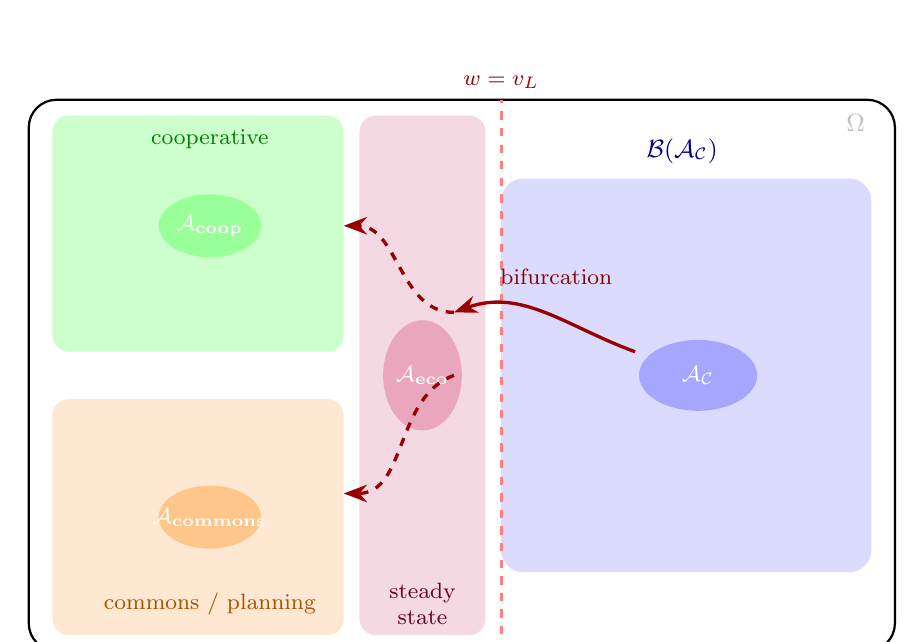
\begin{tikzpicture}[>=Stealth, thick, scale=1.0]
  % Full institutional possibility space Omega
  \draw[thick, rounded corners=10pt] (-5.5,-3.5) rectangle (5.5,3.5);
  \node[gray!50] at (5.0, 3.2) {\small $\Omega$};

  % Capital order basin (currently dominant)
  \fill[blue!14, rounded corners=8pt] (0.5,-2.5) rectangle (5.2,2.5);
  \node[blue!50!black, font=\small] at (2.8, 2.85) {$\mathcal{B}(\mathcal{A}_\mathcal{C})$};
  \fill[blue!35] (3.0, 0) ellipse (0.75cm and 0.45cm);
  \node[white, font=\footnotesize\bfseries] at (3.0, 0) {$\mathcal{A}_\mathcal{C}$};

  % Cooperative attractor
  \fill[green!20, rounded corners=6pt] (-5.2, 0.3) rectangle (-1.5, 3.3);
  \fill[green!40] (-3.2, 1.9) ellipse (0.65cm and 0.4cm);
  \node[white, font=\footnotesize\bfseries] at (-3.2, 1.9) {$\mathcal{A}_{\text{coop}}$};
  \node[green!50!black, font=\footnotesize] at (-3.2, 3.0) {cooperative};

  % Commons attractor
  \fill[orange!18, rounded corners=6pt] (-5.2,-3.3) rectangle (-1.5,-0.3);
  \fill[orange!45] (-3.2,-1.8) ellipse (0.65cm and 0.4cm);
  \node[white, font=\footnotesize\bfseries] at (-3.2,-1.8) {$\mathcal{A}_{\text{commons}}$};
  \node[orange!65!black, font=\footnotesize] at (-3.2,-2.9) {commons / planning};

  % Ecological steady-state attractor
  \fill[purple!15, rounded corners=6pt] (-1.3,-3.3) rectangle (0.3,3.3);
  \fill[purple!35] (-0.5, 0) ellipse (0.5cm and 0.7cm);
  \node[white, font=\footnotesize\bfseries] at (-0.5, 0) {$\mathcal{A}_{\text{eco}}$};
  \node[purple!55!black, font=\footnotesize, align=center] at (-0.5, -2.9) {steady\\state};

  % Boundary w=v_L separating capital from alternatives
  \draw[red!50, very thick, dashed] (0.5,-3.5) -- (0.5, 3.5)
    node[above, red!60!black, font=\footnotesize] {$w = v_L$};

  % Transformation arrows
  \draw[->, very thick, red!60!black]
    (2.2, 0.3) to[out=160, in=20] (-0.1, 0.8);
  \node[red!55!black, font=\footnotesize] at (1.2, 1.25) {bifurcation};

  \draw[->, very thick, red!60!black, dashed]
    (-0.1, 0.8) to[out=180, in=0] (-1.5, 1.9);
  \draw[->, very thick, red!60!black, dashed]
    (-0.1, 0.0) to[out=200, in=0] (-1.5, -1.5);
\end{tikzpicture}
\caption{Post-capitalist institutional geometries as alternative attractors in the full institutional possibility space $\Omega$. The capital order's basin $\mathcal{B}(\mathcal{A}_\mathcal{C})$ occupies the region $w < v_L$ (right of dashed boundary). Beyond the bifurcation boundary lie alternative attractors: cooperative ownership ($\mathcal{A}_{\text{coop}}$), commons-based and planning configurations ($\mathcal{A}_{\text{commons}}$), and ecological steady-state economies ($\mathcal{A}_{\text{eco}}$). Transformation corresponds to driving the trajectory across the bifurcation boundary (red arrows) into the basin of an alternative attractor.}
\label{fig:postcapitalist}
\end{figure}

\subsection{The Constructive Dimension of Transformation}

The geometric representation makes visible a feature of transformation that is often obscured in purely critical political economy: the existence of a viable alternative attractor is a precondition for transformation, not merely a consequence of it. A trajectory that exits $\mathcal{B}(\mathcal{A}_\mathcal{C})$ does not automatically enter the basin of a desirable alternative; it may enter a region of $\Omega$ with no stable attractor at all, corresponding to social disorganization, fragmentation, or authoritarian stabilization under new institutional forms.

This implies that the political project of transformation has two necessary components that must be pursued simultaneously. The first is the destabilizing work: building the social forces and boundary struggles capable of driving $\mu$ across the bifurcation threshold $\mu_c$. The second is the constructive work: building the institutional channels, governance capacities, cooperative enterprises, and cultural frameworks that constitute the alternative attractor $\mathcal{A}'$ in advance of the bifurcation. Without the second, the first produces not transformation but crisis without resolution.

In RSVP terms, the constructive work corresponds to establishing new gradient structures in the social field: creating channels through which value, energy, and meaning can flow under different institutional rules, so that when the old channels are disrupted, the social field can reorganize around the new gradient topology rather than collapsing into disorder.

% ─────────────────────────────────────────────────
\section{Conclusion}
\label{sec:conclusion}

This paper has developed an extended formal reconstruction of political economy drawing on Clara E.\ Mattei, Nancy Fraser, Karl Marx, Karl Polanyi, Thorstein Veblen, Hyman Minsky, Richard Goodwin, Immanuel Wallerstein, and Nicholas Georgescu-Roegen. The methodology throughout has been reconstructive rather than evidentiary: to expose the structural logic of these institutional analyses through dynamical systems theory and the RSVP framework, clarifying their internal architecture and the conditions under which the system could be transformed.

The first movement of the paper, following Mattei, models the capital order as a feedback-stabilized attractor $\mathcal{A}_\mathcal{C}$ within the four-component institutional state space $\mathcal{X}$. The surplus stability region $\mathcal{S} = \{w < v_L\}$ defines the constraint that trajectories must satisfy for capitalist reproduction to continue; the transition map $\Phi$ contains corrective terms implemented through technocratic governance, austerity, and ideological projection. The double-freedom constraint pair formalizes the combination of legal contract freedom with structural exclusion from means of subsistence. The gradient chain $\partial\Pi/\partial u > 0$ gives rigorous content to the claim that unemployment disciplines labor. Austerity implements exponential correction at rate $\lambda$; authoritarian governance reduces the democratic dimensionality $D$ of the accessible policy manifold.

The second movement extends the state space to the socio-ecological configuration $\mathcal{E}_t = (L_t, K_t, R_t, N_t, P_t, I_t)$ and embeds the capital order within the broader institutional architecture described by Fraser. The front-story market economy is sustained by back-story background conditions that the capital order simultaneously deploys and disavows. The disavowal ratio $\delta(t)$ measures the subsidy that the front-story extracts from unaccounted conditions. The accumulation circuit $M \to C \to M'$ imposes the imperative $dM/dt > 0$ and the priority ordering $K_t \succ L_t \succ P_t \succ R_t \succ N_t$. Polanyi's double movement is formalized as a Lotka--Volterra system in the embedding degree $\epsilon$ and counter-movement pressure $Q$. Fraser's four institutional boundaries are projection constraints contested by social movements.

The third movement develops the dynamics of crisis and reproduction. The Goodwin cycle formalizes class dynamics as closed orbits in the $(u, v)$ plane around the stationary point $(u^*, v^*) = (\delta/\gamma, \alpha/\beta)$, interpreting crisis as periodic displacement from the surplus stability region. Minsky's financial instability hypothesis extends the stability region to the augmented space $\hat{\mathcal{S}} = \{w < v_L,\; \lambda < \lambda^*\}$, with the financial amplification coefficient $\sigma_F$ increasing oscillation amplitude during the Ponzi finance phase. Financialization deepens technocracy by extending the temporal horizon of extraction and incorporating bond markets and credit rating agencies as additional components of the feedback controller $\Gamma$. Ideology is formalized as an ideological reproduction operator $\mathcal{H}_t$ that maintains the social conditions under which the restricted possibility space $\Omega_t$ is perceived as the full space $\Omega$. World-system dynamics extend the analysis to a multi-region network $\mathcal{G} = (V, E, W)$ in which core-periphery gradients sustain global surplus extraction through labor arbitrage.

Ecological analysis establishes that the accumulation imperative $dM/dt > 0$ generates irreversible entropy production in the biosphere, formalizing the metabolic rift as $dN_t/dt < 0$ when throughput $\sigma_N(Y_t)$ exceeds renewal capacity $\rho_N(N_t)$. The Irreversibility Proposition establishes that ecological crisis is qualitatively different from other crisis modalities: the entropy produced during ecological depletion cannot be recaptured by reducing output. Ecological constraint therefore deforms the capital order's attractor from within rather than merely displacing trajectories outside the basin.

Boundary struggles are interpreted as bifurcation-seeking perturbations that attempt to shift the control parameter $\mu$ of the institutional dynamical system across a bifurcation point $\mu_c$ at which the qualitative structure of attractors changes. Post-capitalist institutional geometries are represented as alternative attractors in the full possibility space $\Omega$: cooperative ownership shifts the distributional rule toward $w \approx v_L$; public provisioning dissolves the survival-coupling constraint; participatory planning replaces the technocratic control objective with a democratically determined target $\mathcal{S}'$; ecological embedding imposes the steady-state constraint $\rho_N \geq \sigma_N$.

The RSVP framework situates the complete analysis as a controlled non-equilibrium gradient configuration. The capital order maintains the gradient $\nabla(\varrho_K - \varrho_L) > 0$ through institutional channels that prevent spontaneous equilibration; austerity steepens this gradient by counteracting RSVP smoothing dynamics; ideology reduces the curvature of the semantic manifold $\mathcal{S}_{\text{disc}}$; financialization extends the temporal reach of the entropy gradient by drawing on future production; and world-system hierarchy extends the spatial reach of the gradient across the global field $\mathcal{G}$.

The conceptual payoff of the complete framework is a theory of the capital order as a complex social system that is not merely unjust but dynamically structured to reproduce its injustice through interlocking mechanisms operating at economic, political, ideological, financial, global, and ecological scales. Understanding transformation requires understanding all of these mechanisms simultaneously---not only the economic gradient between labor and capital, but the temporal gradient of financial extraction, the spatial gradient of world-system hierarchy, the informational gradient of ideological hegemony, and the thermodynamic gradient of ecological throughput. Mattei identifies who operates the corrective mechanisms; Fraser shows what they destroy in the process; the RSVP framework clarifies what it would mean to construct a social field in which these gradients are organized differently.

% ─────────────────────────────────────────────────
\appendix

\section{Summary of Formal Notations}
\label{app:notation}

\noindent
\begin{tabular}{@{}ll@{}}
  \hline
  \textbf{Symbol} & \textbf{Meaning} \\
  \hline
  \multicolumn{2}{@{}l}{\itshape Institutional state and dynamics} \\
  $\mathcal{C}_t = (L_t, K_t, P_t, I_t)$ & Front-story institutional state at time $t$ \\
  $\mathcal{E}_t = (L_t, K_t, R_t, N_t, P_t, I_t)$ & Socio-ecological state (extended) \\
  $\Phi : \mathcal{X} \to \mathcal{X}$ & Transition map on front-story state space \\
  $\tilde\Phi : \mathcal{Y} \to \mathcal{Y}$ & Transition map on socio-ecological state space \\
  $\mathcal{X},\; \mathcal{Y}$ & Front-story and socio-ecological state spaces \\
  $\mathcal{A}_\mathcal{C}$ & Capital attractor (metastable compact invariant set) \\
  $\mathcal{B}(\mathcal{A}_\mathcal{C})$ & Basin of attraction of the capital order \\
  $\mathcal{S} = \{\mathcal{C} : w < v_L\}$ & Surplus stability region \\
  $\mathcal{M}_\mathcal{C}$ & Capitalist submanifold in $\mathcal{Y}$ \\[4pt]
  \multicolumn{2}{@{}l}{\itshape Labor and distribution} \\
  $w,\; v_L$ & Wage and per-unit value of labor output \\
  $\Pi = v_L - w$ & Surplus; requires $\Pi > 0$ \\
  $S_i,\; w_i$ & Survival requirement and wage of worker $i$ \\
  $W(t),\; S(t)$ & Aggregate wages and aggregate survival threshold \\
  $L_{t+1} = R(L_t, W, S)$ & Labor population reproduction equation \\
  $Y_t = F(K_t, L_t, R_t, N_t, P_t)$ & Extended output with back-story inputs \\
  $\alpha(\mathcal{C}_t) = W/Y$ & Institutionally determined labor share \\
  $B_L(u, \theta)$ & Labor bargaining power \\
  $u(t)$ & Unemployment rate \\
  $\partial\Pi/\partial u > 0$ & Unemployment–profit gradient chain \\
  $\lambda$ & Austerity correction rate \\[4pt]
  \multicolumn{2}{@{}l}{\itshape Double freedom and accumulation} \\
  $\mathcal{D}$ & Double-freedom region of institutional state space \\
  $M \to C \to M'$ & Capital circuit; $M' = M + \Pi$ \\
  $dM/dt > 0$ & Accumulation imperative \\
  $\delta(t)$ & Disavowal ratio (fraction of output from unaccounted conditions) \\[4pt]
  \multicolumn{2}{@{}l}{\itshape Background conditions and crisis} \\
  $R_t,\; N_t$ & Social reproduction and ecological systems \\
  $B_t = (R_t, N_t, P_t)$ & Background condition vector \\
  $B^*$ & Structural crisis threshold \\
  $\rho(B_t)$ & Natural renewal rate of background conditions \\
  $\epsilon(t)$ & Market embedding degree \\
  $Q(t)$ & Counter-movement pressure amplitude \\[4pt]
  \multicolumn{2}{@{}l}{\itshape Boundary projections} \\
  $\pi_M,\; \pi_{M/R},\; \pi_{M/P},\; \pi_{M/N}$ & Standard and boundary projection operators \\
  $\pi_{exp}$ & Expropriation-hiding projection \\[4pt]
  \multicolumn{2}{@{}l}{\itshape Informational and technocratic mechanisms} \\
  $\Omega,\; \Omega_t$ & Full and historically restricted institutional possibility spaces \\
  $\mathcal{P}_t : \Omega \to \Omega_t$ & Time-indexed neoclassical projection operator \\
  $X_t = (u,\pi,g,r,B_L)$ & Observable macroeconomic state vector \\
  $P_t = \Gamma(X_t)$ & Technocratic feedback controller \\
  $\mathcal{M}_D,\; D$ & Policy manifold and its democratic dimensionality \\
  $E_{\mathrm{pub}}(t)$ & Public expenditure energy injection \\[4pt]
  \multicolumn{2}{@{}l}{\itshape RSVP field theory} \\
  $\varrho_L,\; \varrho_K,\; \varrho_N,\; \varrho_R$ & Entropy density fields (labor, capital, ecology, reproduction) \\
  $\mathbf{v},\; \sigma$ & RSVP smoothing flux and entropy production rate \\
  $\mathcal{S}_{\mathrm{disc}}$ & Semantic manifold of economic discourse \\
  $\kappa(\mathcal{S}_{\mathrm{disc}})$ & Curvature tensor of semantic manifold \\[4pt]
  \multicolumn{2}{@{}l}{\itshape Institutional potential landscape} \\
  $V : \mathcal{X} \to \mathbb{R}_{\geq 0}$ & Institutional potential (Lyapunov function) \\
  $V(x) = \tfrac{1}{2}k x^2$ & Quadratic potential; $k$ = stiffness of restoring force \\
  $\dot x = -\lambda \nabla V$ & Gradient descent (austerity as restoring force) \\
  $F_{\text{dem}}(t)$ & Democratic pressure force \\
  $\text{Hess}(V)$ & Hessian of potential; larger under austerity \\[4pt]
  \multicolumn{2}{@{}l}{\itshape Crisis cycles and finance} \\
  $(u^*, v^*) = (\delta/\gamma, \alpha/\beta)$ & Goodwin stationary point \\
  $H(u,v)$ & Conserved quantity of the Goodwin system \\
  $Z_t = (d_t, a_t, \lambda_t)$ & Financial state vector (debt, assets, leverage) \\
  $\hat{X}_t = (K_t, L_t, Z_t)$ & Augmented economic-financial state \\
  $\lambda^*$ & Financial leverage crisis threshold \\
  $\sigma_F$ & Financial amplification coefficient \\
  $\hat{\mathcal{S}} = \{w < v_L,\, \lambda < \lambda^*\}$ & Augmented stability region \\[4pt]
  \multicolumn{2}{@{}l}{\itshape Ideology and world system} \\
  $\mathcal{H}_t : \mathcal{I} \to \mathcal{I}$ & Ideological reproduction operator \\
  $\Omega_{\text{legitimate}} \subset \Omega$ & Ideologically admissible institutional domain \\
  $\mathcal{G} = (V, E, W)$ & World-system weighted directed graph \\
  $w_c,\; w_p$ & Core and peripheral wages \\
  $\Delta_{\min}$ & Minimum wage differential for labor arbitrage \\[4pt]
  \multicolumn{2}{@{}l}{\itshape Ecological thermodynamics} \\
  $\rho_N(N_t)$ & Ecological renewal rate \\
  $\sigma_N(Y_t)$ & Entropy production rate of economic throughput \\[4pt]
  \multicolumn{2}{@{}l}{\itshape Phase transitions and post-capitalism} \\
  $\mu,\; \mu_c$ & Control parameter and bifurcation threshold \\
  $\mathcal{A}_{\text{coop}},\; \mathcal{A}_{\text{commons}},\; \mathcal{A}_{\text{eco}}$ & Alternative post-capitalist attractors \\
  $D_I(L_t, P_t)$ & Democratic investment function \\
  \hline
\end{tabular}

% ─────────────────────────────────────────────────
\section{The Goodwin Model of Class Dynamics}
\label{app:goodwin}

Richard Goodwin's 1967 contribution to formal political economy represents one of the most elegant attempts to model the cyclical dynamics of capitalism with minimal formal machinery. By adapting the Lotka--Volterra equations of mathematical ecology, Goodwin showed that the interaction between employment and the wage share naturally generates recurrent oscillations rather than convergence to a stable equilibrium---a formal result that supports the broader claim of this paper that the capital order is reproduced through structured instability rather than harmonious equilibrium.

The system~\eqref{eq:goodwin_u}--\eqref{eq:goodwin_v} admits a conserved quantity analogous to the Lotka--Volterra integral of motion:
\begin{equation}
  H(u,v) = \gamma u - \delta \ln u + \beta v - \alpha \ln v = \text{const.}
\end{equation}
The level curves of $H$ are closed orbits in the $(u,v)$ plane, confirming that the Goodwin system generates perpetual cycles rather than converging to $(u^*, v^*)$. Each orbit encloses the stationary point, and initial conditions determine which orbit the system inhabits.

The model is of course severely simplified: it abstracts from credit, state policy, ecological limits, reproductive labor, and global asymmetries. Its value is heuristic. Even at maximal simplification---two variables, four parameters---the class interaction between employment and the wage share generates recurrent destabilization. This demonstrates that cyclical dynamics are endogenous to the capital-labor relation rather than imposed by external disturbances.

The Goodwin cycle relates directly to the Minsky financial cycle analyzed in Section~\ref{sec:crisis_cycles}. The labor-market cycle operates on a shorter timescale (the business cycle) while financial cycles operate on a longer timescale (the credit cycle). Their interaction produces the multi-frequency oscillatory dynamics characteristic of actually observed capitalist economies. When both cycles peak simultaneously---full employment driving up wages while leverage approaches $\lambda^*$---the combined displacement from the stability region is sufficient to trigger major structural crises of the 1929 or 2008 variety.

% ─────────────────────────────────────────────────
\section{Phase Portrait of the Goodwin Cycle}
\label{app:goodwin_phase}

The phase portrait below provides a stylized representation of the closed orbits generated by the Goodwin system. The nullclines $v = \alpha/\beta$ and $u = \delta/\gamma$ divide the phase plane into four quadrants with distinct direction fields. The system circulates counterclockwise: from the lower-right quadrant (high employment, low wages, rising profits) through the upper-right (high employment, rising wages, falling profits) to the upper-left (falling employment, high wages, further falling profits) and back through the lower-left (low employment, falling wages, recovering profits) to the lower-right.

This cycle corresponds precisely to the Mattei pattern: phases of labor strengthening are repeatedly followed by institutional countermeasures that restore profitability and reimpose discipline. The formal model makes visible the mechanism through which this recurrence is structurally guaranteed: not by conspiracy or contingency, but by the endogenous dynamics of the wage-employment interaction.

\begin{figure}[ht]
\centering
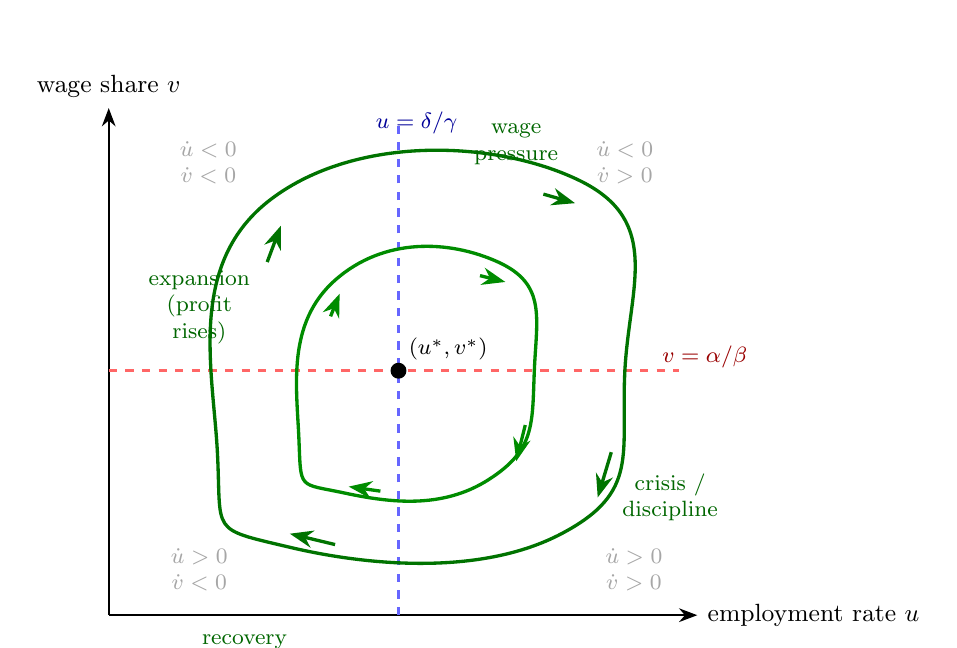
\begin{tikzpicture}[>=Stealth, thick, scale=1.15]
  \draw[->] (0,0) -- (6.5,0) node[right] {\small employment rate $u$};
  \draw[->] (0,0) -- (0,5.6) node[above] {\small wage share $v$};

  % Nullclines
  \draw[red!60, dashed, very thick] (0, 2.7) -- (6.3, 2.7);
  \node[red!60!black, font=\footnotesize, right] at (6.0, 2.85) {$v = \alpha/\beta$};
  \draw[blue!60, dashed, very thick] (3.2, 0) -- (3.2, 5.4);
  \node[blue!60!black, font=\footnotesize, above] at (3.4, 5.2) {$u = \delta/\gamma$};

  % Equilibrium
  \fill (3.2, 2.7) circle (2.5pt);
  \node[font=\footnotesize, above right] at (3.2, 2.7) {$(u^*, v^*)$};

  % Outer orbit
  \draw[green!45!black, very thick]
    plot[smooth cycle, tension=0.85] coordinates {
      (1.2,1.8) (1.8,4.6) (5.2,4.8) (5.7,2.7)
      (5.0,0.9) (2.0,0.75)};
  \draw[->, green!45!black, very thick] (1.75,3.9) -- (1.9,4.3);
  \draw[->, green!45!black, very thick] (4.8,4.65) -- (5.15,4.55);
  \draw[->, green!45!black, very thick] (5.55,1.8) -- (5.4,1.3);
  \draw[->, green!45!black, very thick] (2.5,0.78) -- (2.0,0.9);

  % Inner orbit
  \draw[green!55!black, very thick]
    plot[smooth cycle, tension=0.88] coordinates {
      (2.1,1.95) (2.5,3.7) (4.3,3.9) (4.7,2.7)
      (4.2,1.5) (2.6,1.35)};
  \draw[->, green!55!black, very thick] (2.45,3.3) -- (2.55,3.55);
  \draw[->, green!55!black, very thick] (4.1,3.75) -- (4.38,3.68);
  \draw[->, green!55!black, very thick] (4.6,2.1) -- (4.5,1.7);
  \draw[->, green!55!black, very thick] (3.0,1.37) -- (2.65,1.42);

  % Quadrant labels
  \node[font=\footnotesize, align=center, gray!70] at (1.1, 5.0) {$\dot u<0$\\$\dot v<0$};
  \node[font=\footnotesize, align=center, gray!70] at (5.7, 5.0) {$\dot u<0$\\$\dot v>0$};
  \node[font=\footnotesize, align=center, gray!70] at (5.8, 0.5) {$\dot u>0$\\$\dot v>0$};
  \node[font=\footnotesize, align=center, gray!70] at (1.0, 0.5) {$\dot u>0$\\$\dot v<0$};

  % Phase labels on orbit
  \node[green!40!black, font=\footnotesize, align=center] at (1.0, 3.4)
    {expansion\\(profit\\rises)};
  \node[green!40!black, font=\footnotesize, align=center] at (4.5, 5.2)
    {wage\\pressure};
  \node[green!40!black, font=\footnotesize, align=center] at (6.2, 1.3)
    {crisis /\\discipline};
  \node[green!40!black, font=\footnotesize, align=center] at (1.5, -0.3)
    {recovery};
\end{tikzpicture}
\caption{Phase portrait of the Goodwin cycle. Two representative closed orbits (inner and outer) circulate counterclockwise around the stationary point $(u^*, v^*)$. The quadrant labels indicate the sign of $\dot u$ and $\dot v$ in each region. The cycle passes through four phases: profit recovery (lower-left), expansion (upper-left), wage pressure compressing surplus (upper-right), and disciplinary crisis restoring profitability (lower-right). The Goodwin model demonstrates that cyclical class dynamics are endogenous to the wage-employment interaction.}
\label{fig:goodwin_phase}
\end{figure}

% ─────────────────────────────────────────────────
\section{Institutional Attractors and Transformation Geometry}
\label{app:attractors}

The main formal claim of this paper is that capitalism corresponds to a particular configuration of institutional constraints and that transformation corresponds to a redefinition of those constraints. This appendix makes the geometric content of that claim explicit.

The full institutional possibility space $\Omega$ is a high-dimensional manifold whose points represent all conceivable arrangements of property rights, production organization, distribution mechanisms, governance structures, and ideological frameworks. The capital order occupies a specific connected region of $\Omega$ defined by the intersection of the surplus stability condition and the background viability conditions:
\begin{equation}
  \mathcal{M}_\mathcal{C} = \bigl\{\, \mathcal{E} \in \mathcal{Y} : w < v_L,\;\; B \geq B^*,\;\; \lambda < \lambda^* \,\bigr\}.
\end{equation}
The three constraints---distributional, ecological-reproductive, and financial---define three boundary surfaces of $\mathcal{M}_\mathcal{C}$. The capital order can exit through any of these surfaces, corresponding to a wage-driven crisis ($w \to v_L$), a structural background-conditions crisis ($B \to B^*$), or a financial crisis ($\lambda \to \lambda^*$).

Post-capitalist configurations correspond to other connected regions of $\Omega$ with different constraint structures. They are not accessible by continuous deformation within $\mathcal{M}_\mathcal{C}$; they require crossing one or more of the boundary surfaces. Social transformation is therefore a topological operation: it changes the connectivity of the region that institutional trajectories inhabit, rather than merely adjusting the coordinates of trajectories within a fixed region.

The RSVP perspective adds a thermodynamic dimension to this picture. The capital order is a non-equilibrium steady state maintained by continuous institutional work against the natural RSVP smoothing dynamics. Each alternative configuration is also a non-equilibrium steady state, but one organized around different gradient structures. The constructive dimension of transformation---building cooperative enterprises, public institutions, commons governance, ecological constraints---is the work of establishing the new gradient topology in advance of the bifurcation. Without this preparatory construction, the exit from $\mathcal{M}_\mathcal{C}$ does not lead to an alternative attractor; it leads to a region of $\Omega$ with no stable configuration, which is the dynamical analogue of social collapse.

\newpage

% ─────────────────────────────────────────────────
\begin{thebibliography}{99}

\bibitem{Mattei2024}
Mattei, Clara E. (2024).
\textit{Escape from Capitalism: An Intervention}.
New York: Simon \& Schuster.

\bibitem{Mattei2022}
Mattei, Clara E. (2022).
\textit{The Capital Order: How Economists Invented Austerity and Paved the Way to Fascism}.
Chicago: University of Chicago Press.

\bibitem{Marx1867}
Marx, Karl (1867).
\textit{Capital: A Critique of Political Economy, Volume~I}.
Hamburg: Otto Meissner Verlag.

\bibitem{Polanyi1944}
Polanyi, Karl (1944).
\textit{The Great Transformation: The Political and Economic Origins of Our Time}.
Boston: Beacon Press.

\bibitem{Fraser2022}
Fraser, Nancy (2022).
\textit{Cannibal Capitalism: How Our System Is Devouring Democracy, Care, and the Planet---and What We Can Do About It}.
London: Verso.

\bibitem{Fraser2014}
Fraser, Nancy (2014).
Behind Marx's Hidden Abode: For an Expanded Conception of Capitalism.
\textit{New Left Review}, 86, 55--72.

\bibitem{Veblen1899}
Veblen, Thorstein (1899).
\textit{The Theory of the Leisure Class}.
New York: Macmillan.

\bibitem{Veblen1904}
Veblen, Thorstein (1904).
\textit{The Theory of Business Enterprise}.
New York: Charles Scribner's Sons.

\bibitem{Harvey2010}
Harvey, David (2010).
\textit{The Enigma of Capital and the Crises of Capitalism}.
Oxford: Oxford University Press.

\bibitem{Harvey2014}
Harvey, David (2014).
\textit{Seventeen Contradictions and the End of Capitalism}.
Oxford: Oxford University Press.

\bibitem{Arrighi1994}
Arrighi, Giovanni (1994).
\textit{The Long Twentieth Century}.
London: Verso.

\bibitem{Braudel1982}
Braudel, Fernand (1982).
\textit{Civilization and Capitalism, 15th--18th Century, Volume~II: The Wheels of Commerce}.
New York: Harper \& Row.

\bibitem{Minsky1986}
Minsky, Hyman P. (1986).
\textit{Stabilizing an Unstable Economy}.
New Haven: Yale University Press.

\bibitem{Goodwin1967}
Goodwin, Richard M. (1967).
A Growth Cycle.
In C.~H.~Feinstein (ed.), \textit{Socialism, Capitalism and Economic Growth}.
Cambridge: Cambridge University Press.

\bibitem{Strogatz2015}
Strogatz, Steven H. (2015).
\textit{Nonlinear Dynamics and Chaos}.
Boulder: Westview Press.

\bibitem{Georgescu1971}
Georgescu-Roegen, Nicholas (1971).
\textit{The Entropy Law and the Economic Process}.
Cambridge, MA: Harvard University Press.

\bibitem{Daly1996}
Daly, Herman (1996).
\textit{Beyond Growth: The Economics of Sustainable Development}.
Boston: Beacon Press.

\bibitem{Moore2015}
Moore, Jason W. (2015).
\textit{Capitalism in the Web of Life}.
London: Verso.

\bibitem{Federici2012}
Federici, Silvia (2012).
\textit{Revolution at Point Zero: Housework, Reproduction, and Feminist Struggle}.
Oakland: PM Press.

\bibitem{Bhattacharya2017}
Bhattacharya, Tithi (ed.) (2017).
\textit{Social Reproduction Theory}.
London: Pluto Press.

\bibitem{Piketty2014}
Piketty, Thomas (2014).
\textit{Capital in the Twenty-First Century}.
Cambridge, MA: Harvard University Press.

\bibitem{Wallerstein2004}
Wallerstein, Immanuel (2004).
\textit{World-Systems Analysis: An Introduction}.
Durham: Duke University Press.

\bibitem{North1990}
North, Douglass C. (1990).
\textit{Institutions, Institutional Change and Economic Performance}.
Cambridge: Cambridge University Press.

\bibitem{Ostrom1990}
Ostrom, Elinor (1990).
\textit{Governing the Commons}.
Cambridge: Cambridge University Press.

\bibitem{Keynes1936}
Keynes, John Maynard (1936).
\textit{The General Theory of Employment, Interest and Money}.
London: Macmillan.

\bibitem{Gramsci1971}
Gramsci, Antonio (1971).
\textit{Selections from the Prison Notebooks}.
Edited and translated by Q.\ Hoare and G.\ N.\ Smith.
London: Lawrence \& Wishart.

\bibitem{Minsky1992}
Minsky, Hyman P. (1992).
The Financial Instability Hypothesis.
Working Paper No.~74. Annandale-on-Hudson: Levy Economics Institute.

\bibitem{Keen1995}
Keen, Steve (1995).
Finance and Economic Breakdown: Modelling Minsky's Financial Instability Hypothesis.
\textit{Journal of Post Keynesian Economics}, 17(4), 607--635.

\end{thebibliography}

\end{document}
